\newpage

\onecolumn

\appendix

\section{Oszilloskop-Bilder}
\label{sec:plots}
\begin{figure}[htbp]
\begin{center}
  \subfloat[Photomultiplier 1]{
    \label{fig:photomultiplier_1}
    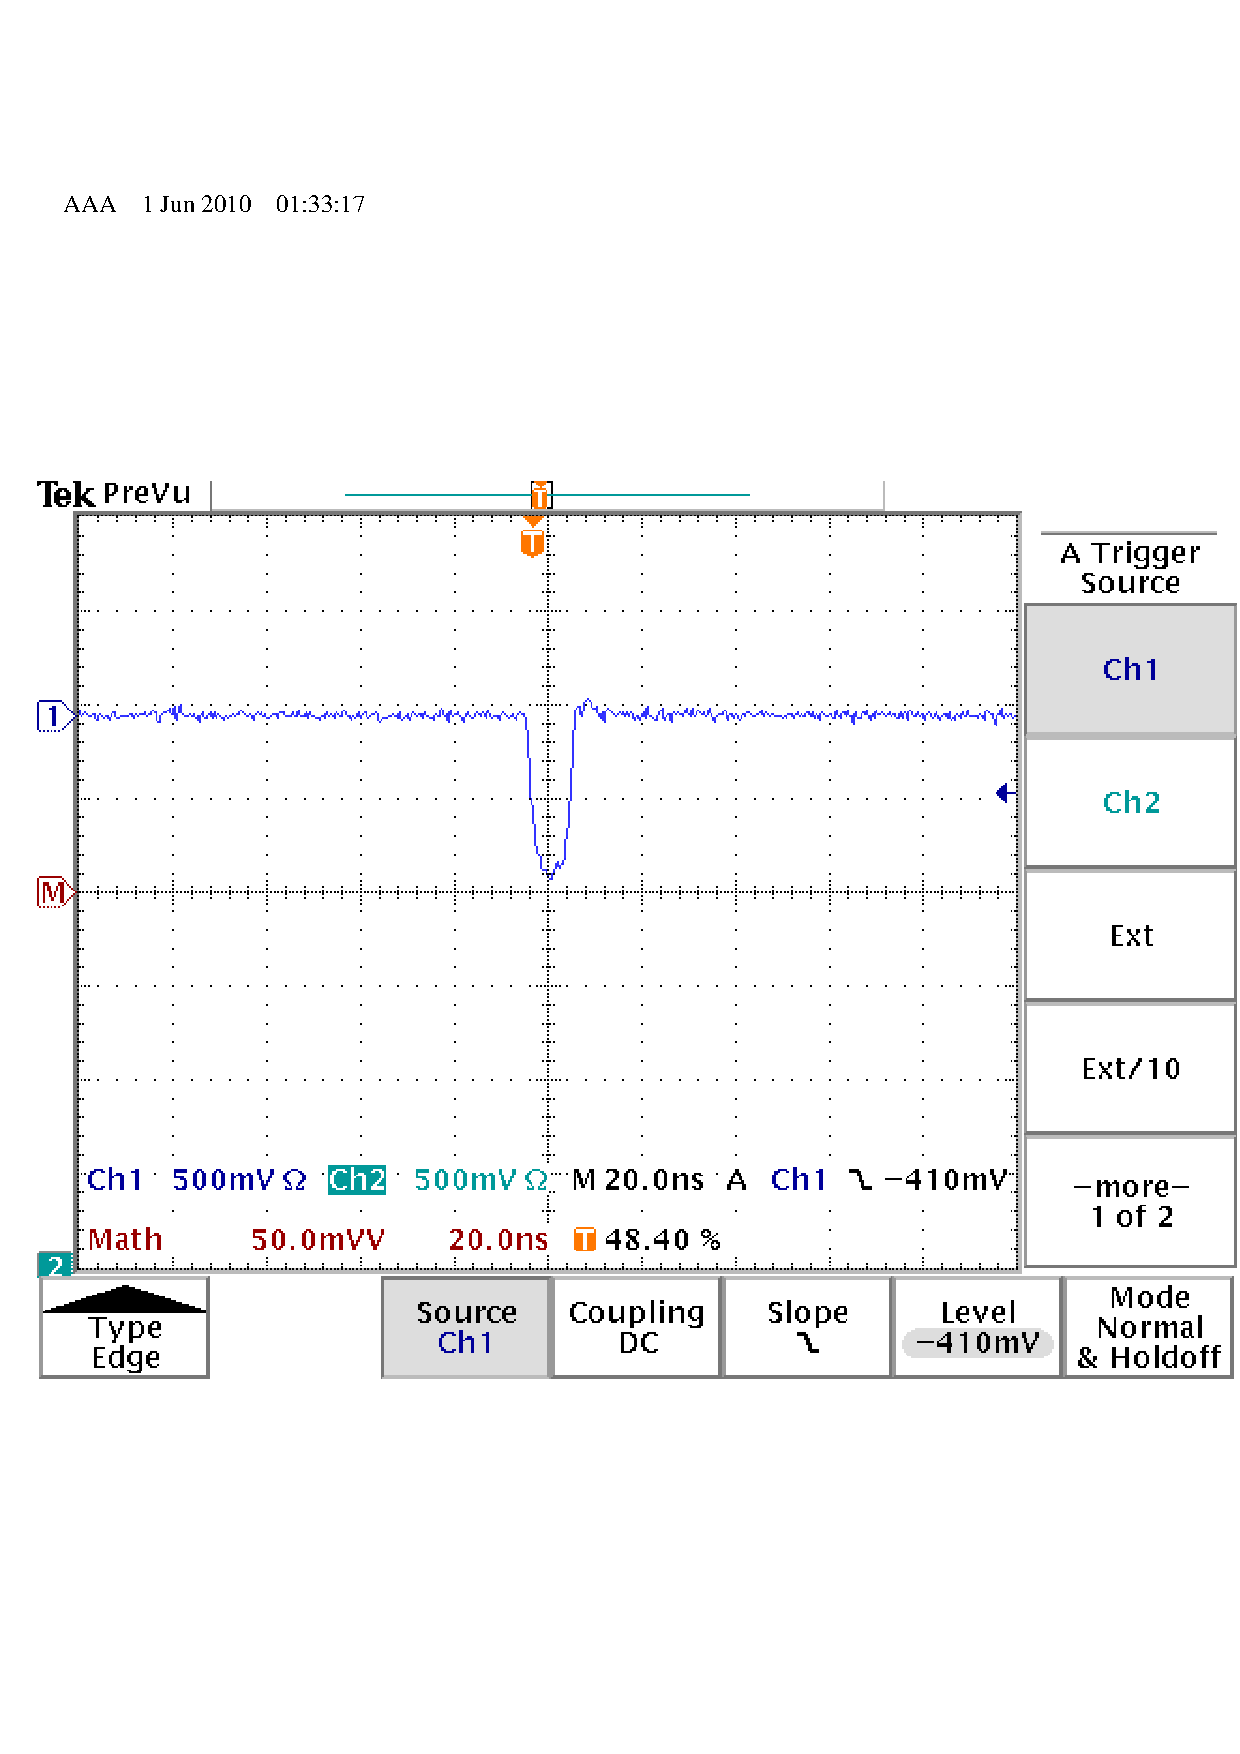
\includegraphics[width=0.45\textwidth,keepaspectratio,viewport=0 52 472 436,clip]{../tmp/TEK00013.pdf}}
  \subfloat[Photomultiplier 2]{
    \label{fig:photomultiplier_2}
    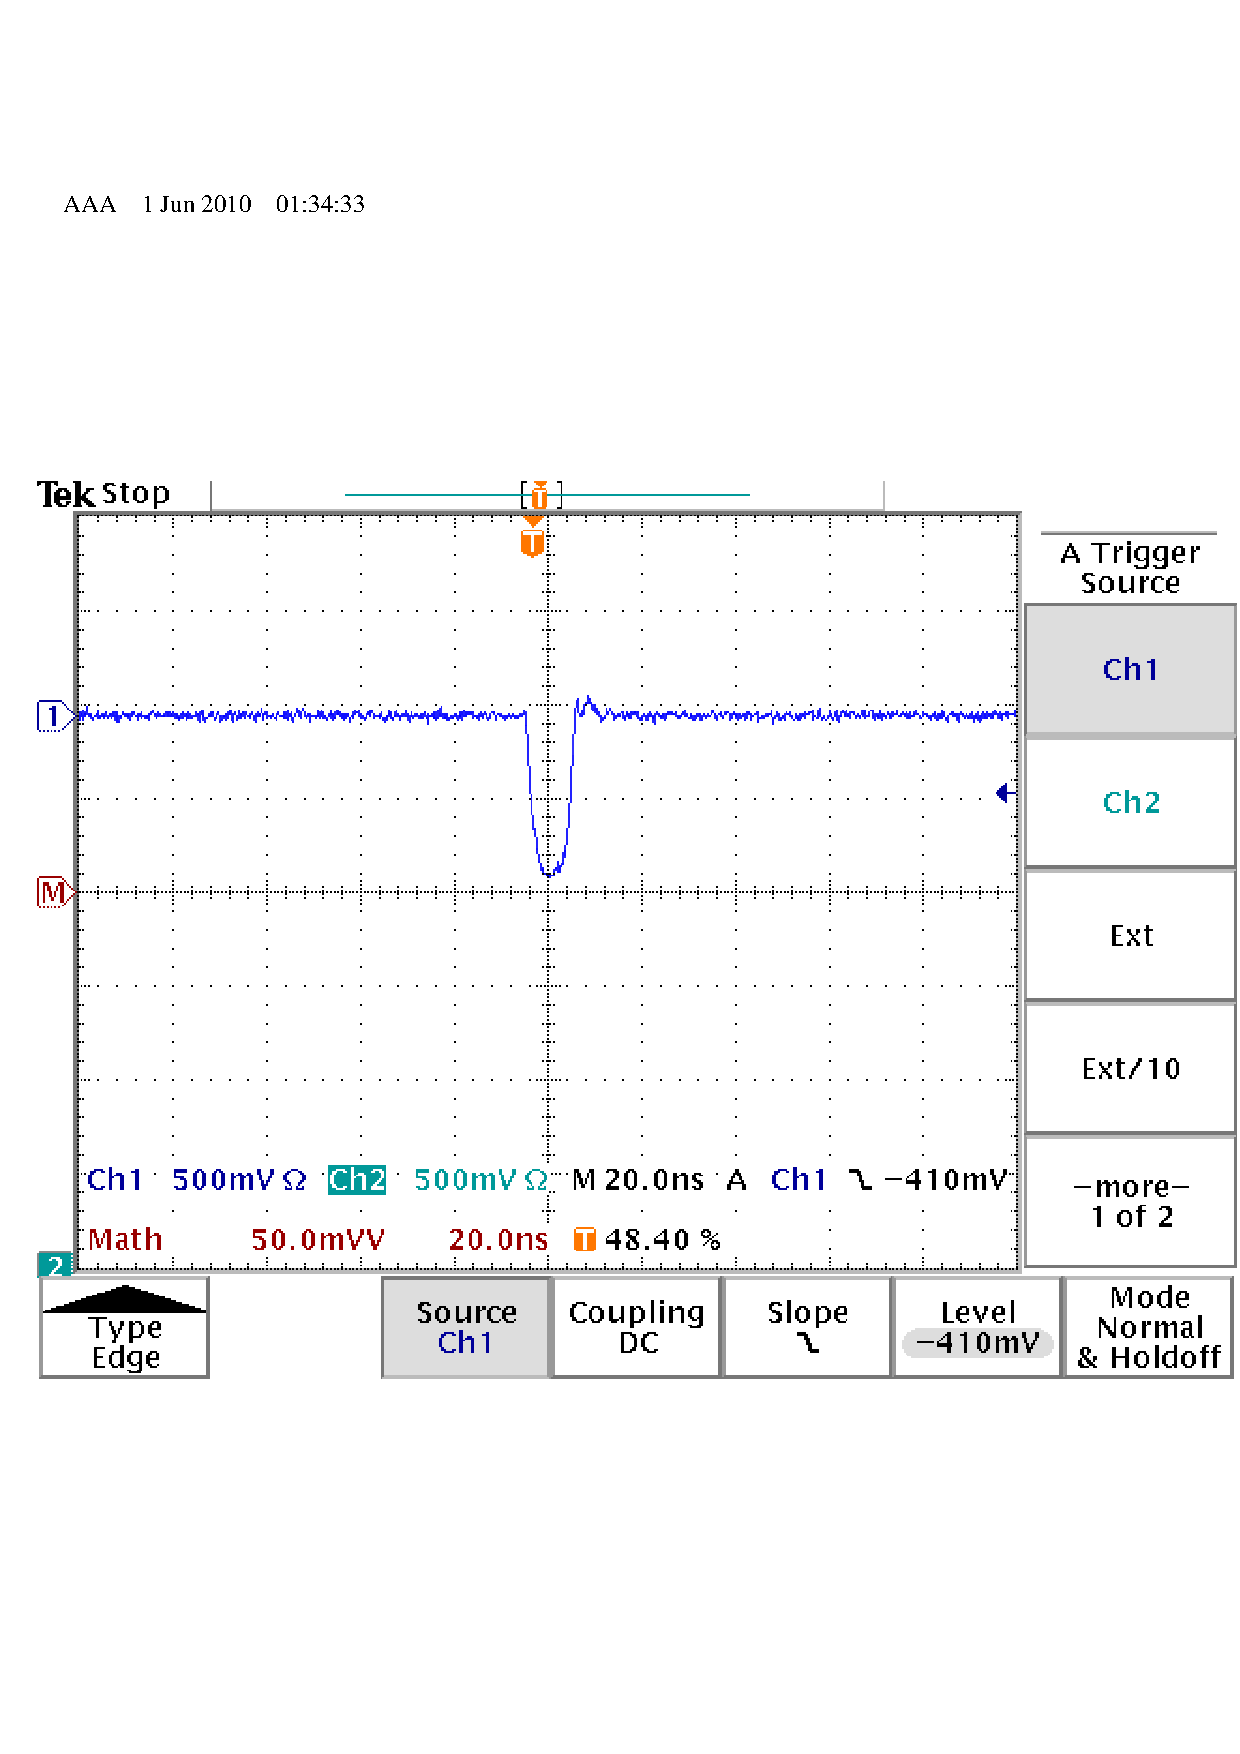
\includegraphics[width=0.45\textwidth,keepaspectratio,viewport=0 52 472 436,clip]{../tmp/TEK00014.pdf}
  }
  \newline
  \subfloat[Photomultiplier 3]{
    \label{fig:photomultiplier_3}
    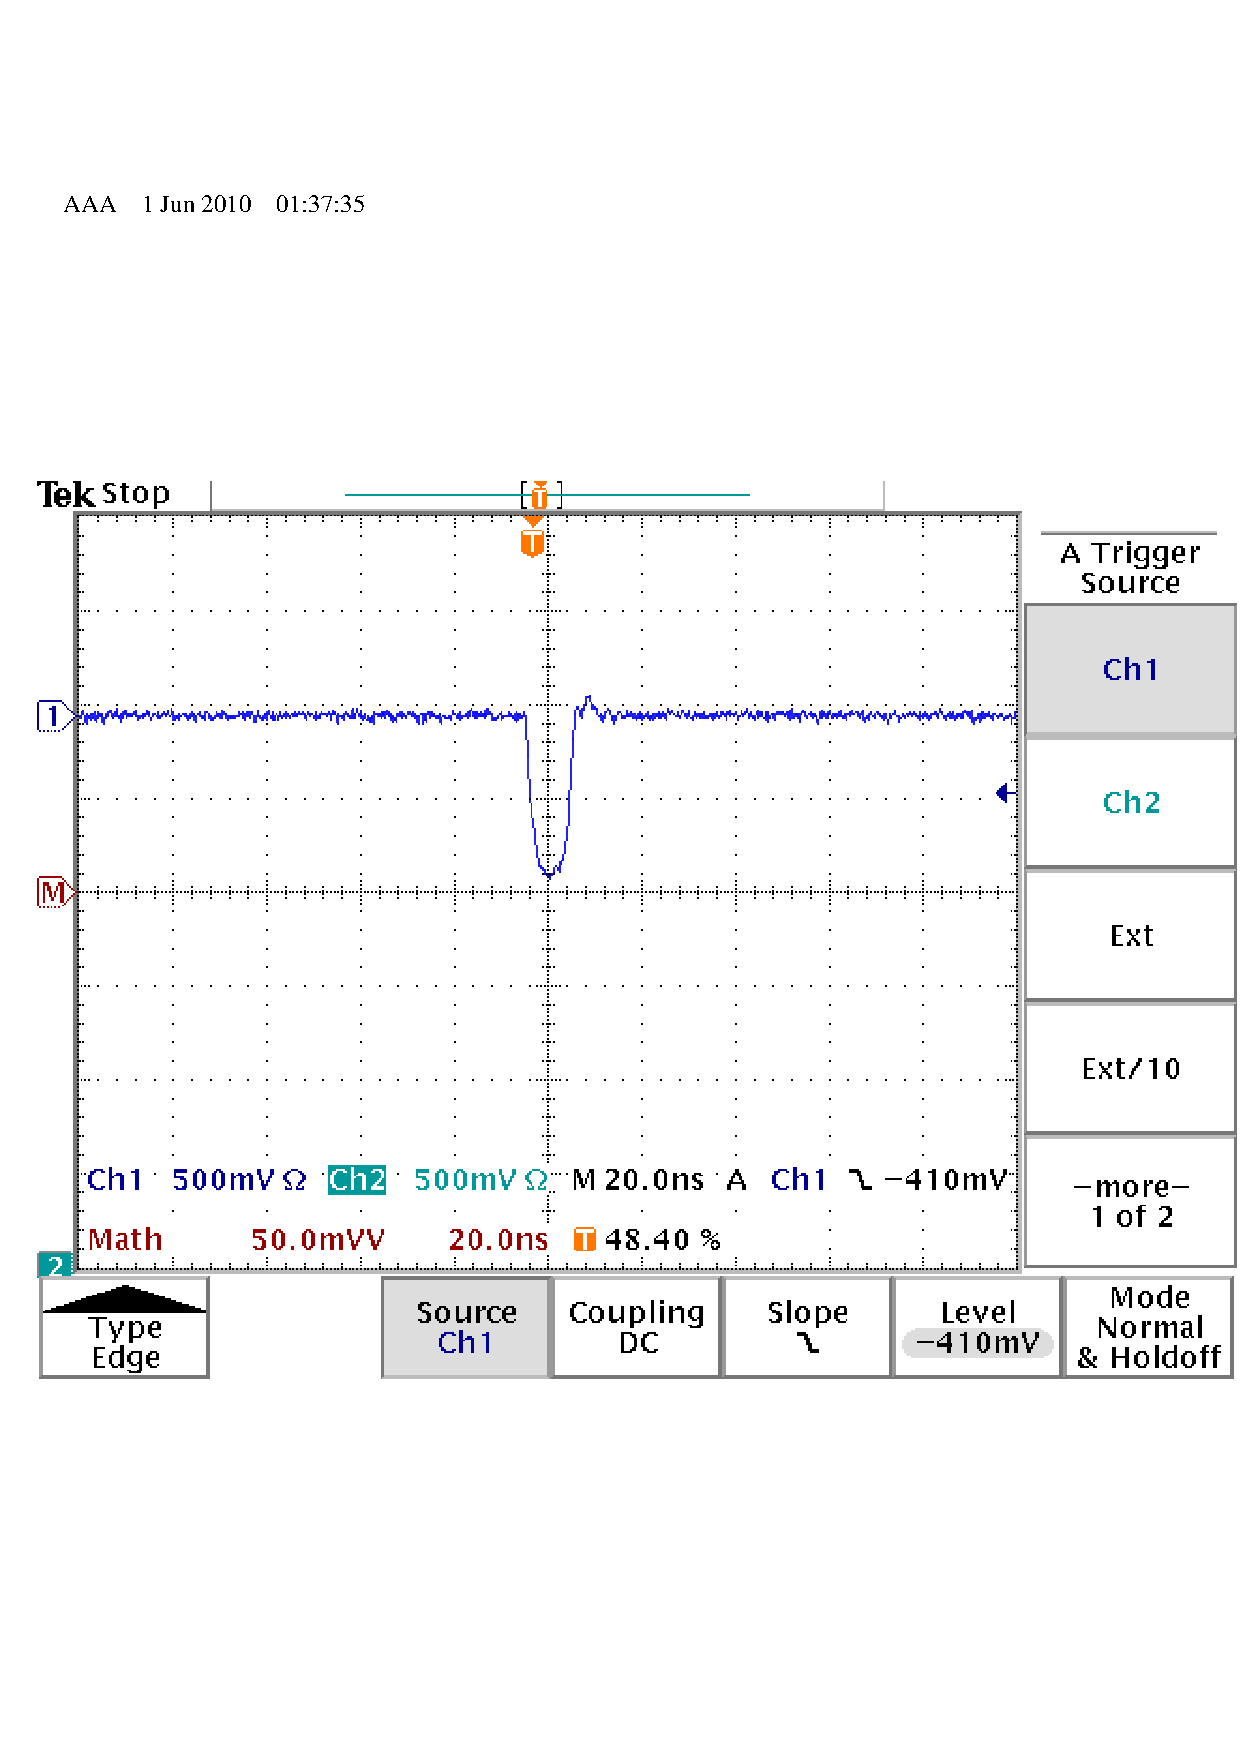
\includegraphics[width=0.45\textwidth,keepaspectratio,viewport=0 52 472 436,clip]{../tmp/TEK00015.pdf}
  }
  \subfloat[Photomultiplier 4]{
    \label{fig:photomultiplier_4}
    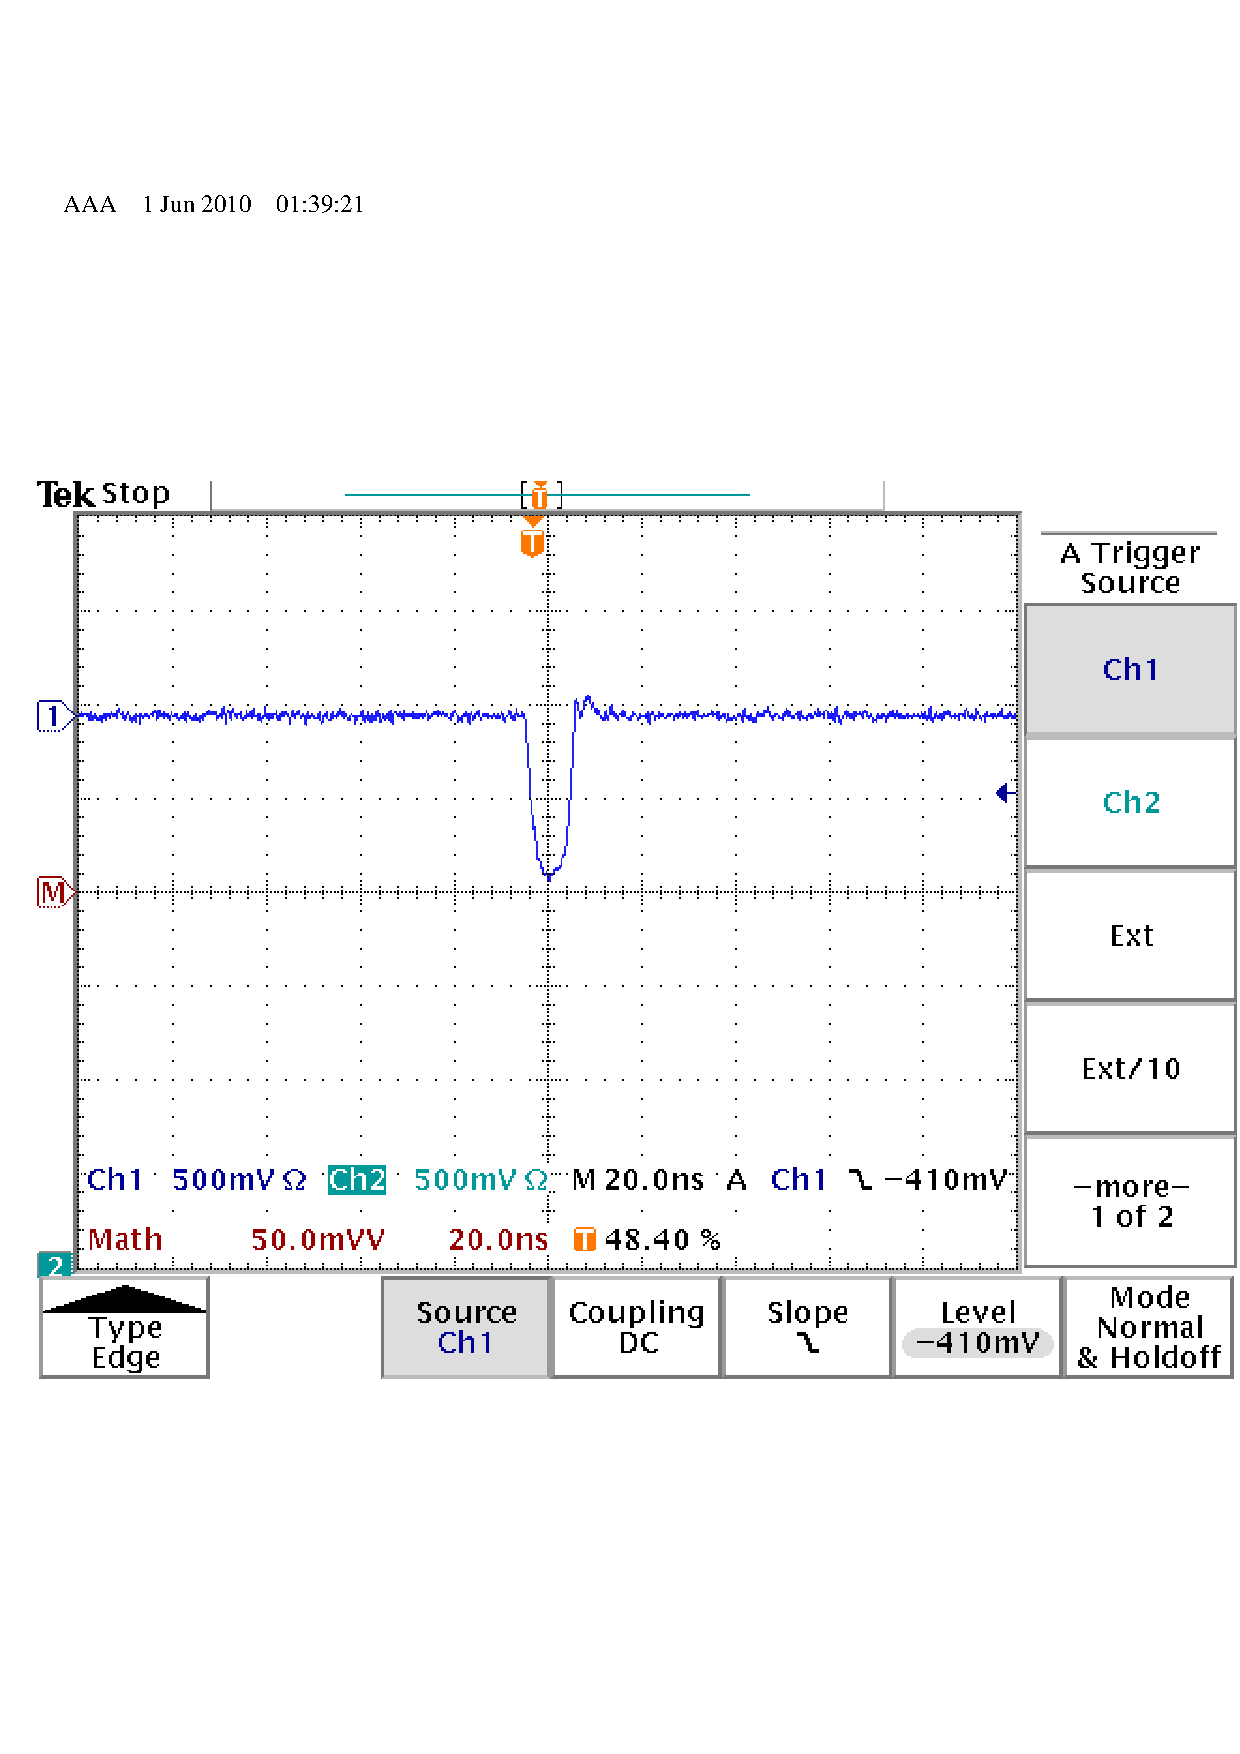
\includegraphics[width=0.45\textwidth,keepaspectratio,viewport=0 52 472 436,clip]{../tmp/TEK00016.pdf}
  }
  \newline
  \subfloat[Photomultiplier 5]{
    \label{fig:photomultiplier_5}
    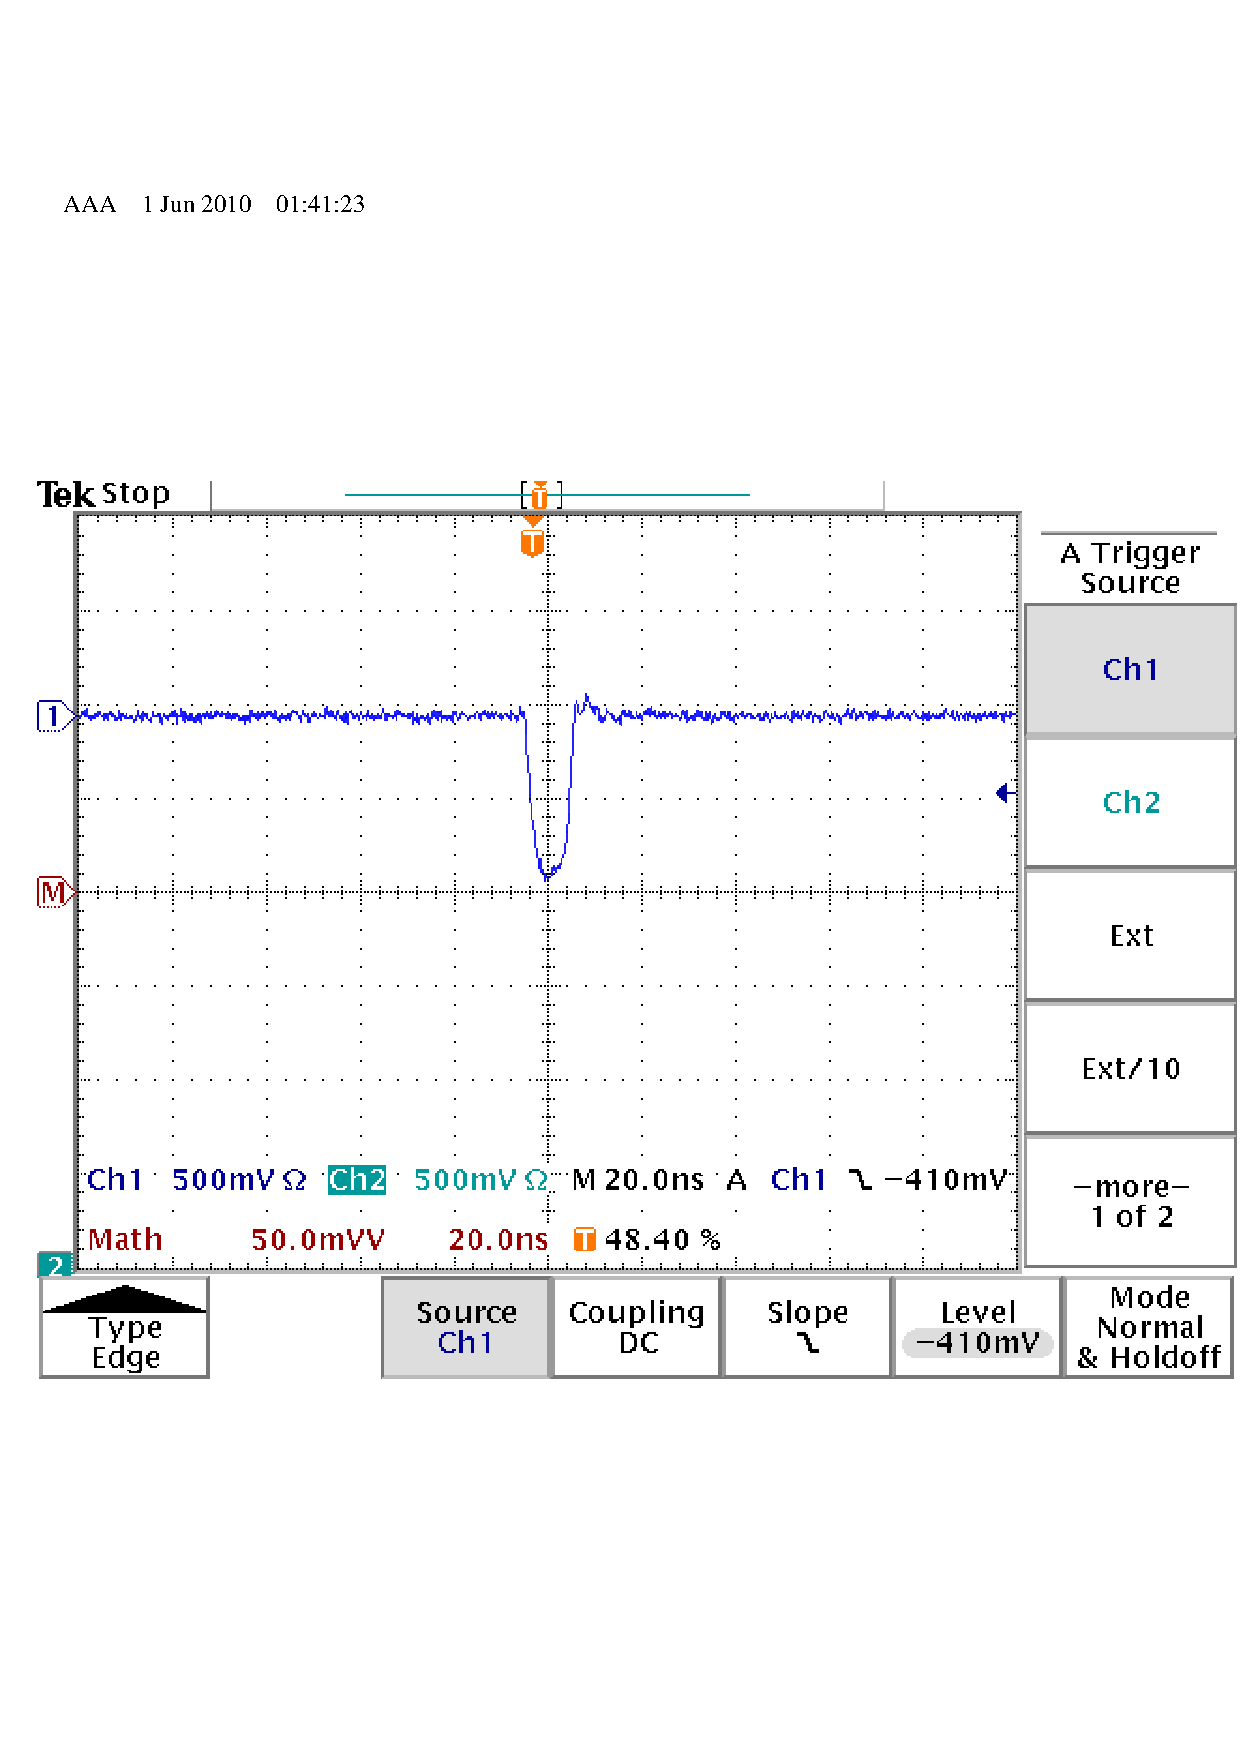
\includegraphics[width=0.45\textwidth,keepaspectratio,viewport=0 52 472 436,clip]{../tmp/TEK00017.pdf}
  }
  \caption{Signale in den einzelnen Photomultipliern}
  \label{fig:PMs}
\end{center}
\end{figure}

\begin{figure}[htbp]
\begin{center}
  \subfloat[Zeitdifferenz 1]{
    \label{fig:zeitdiff_1}
    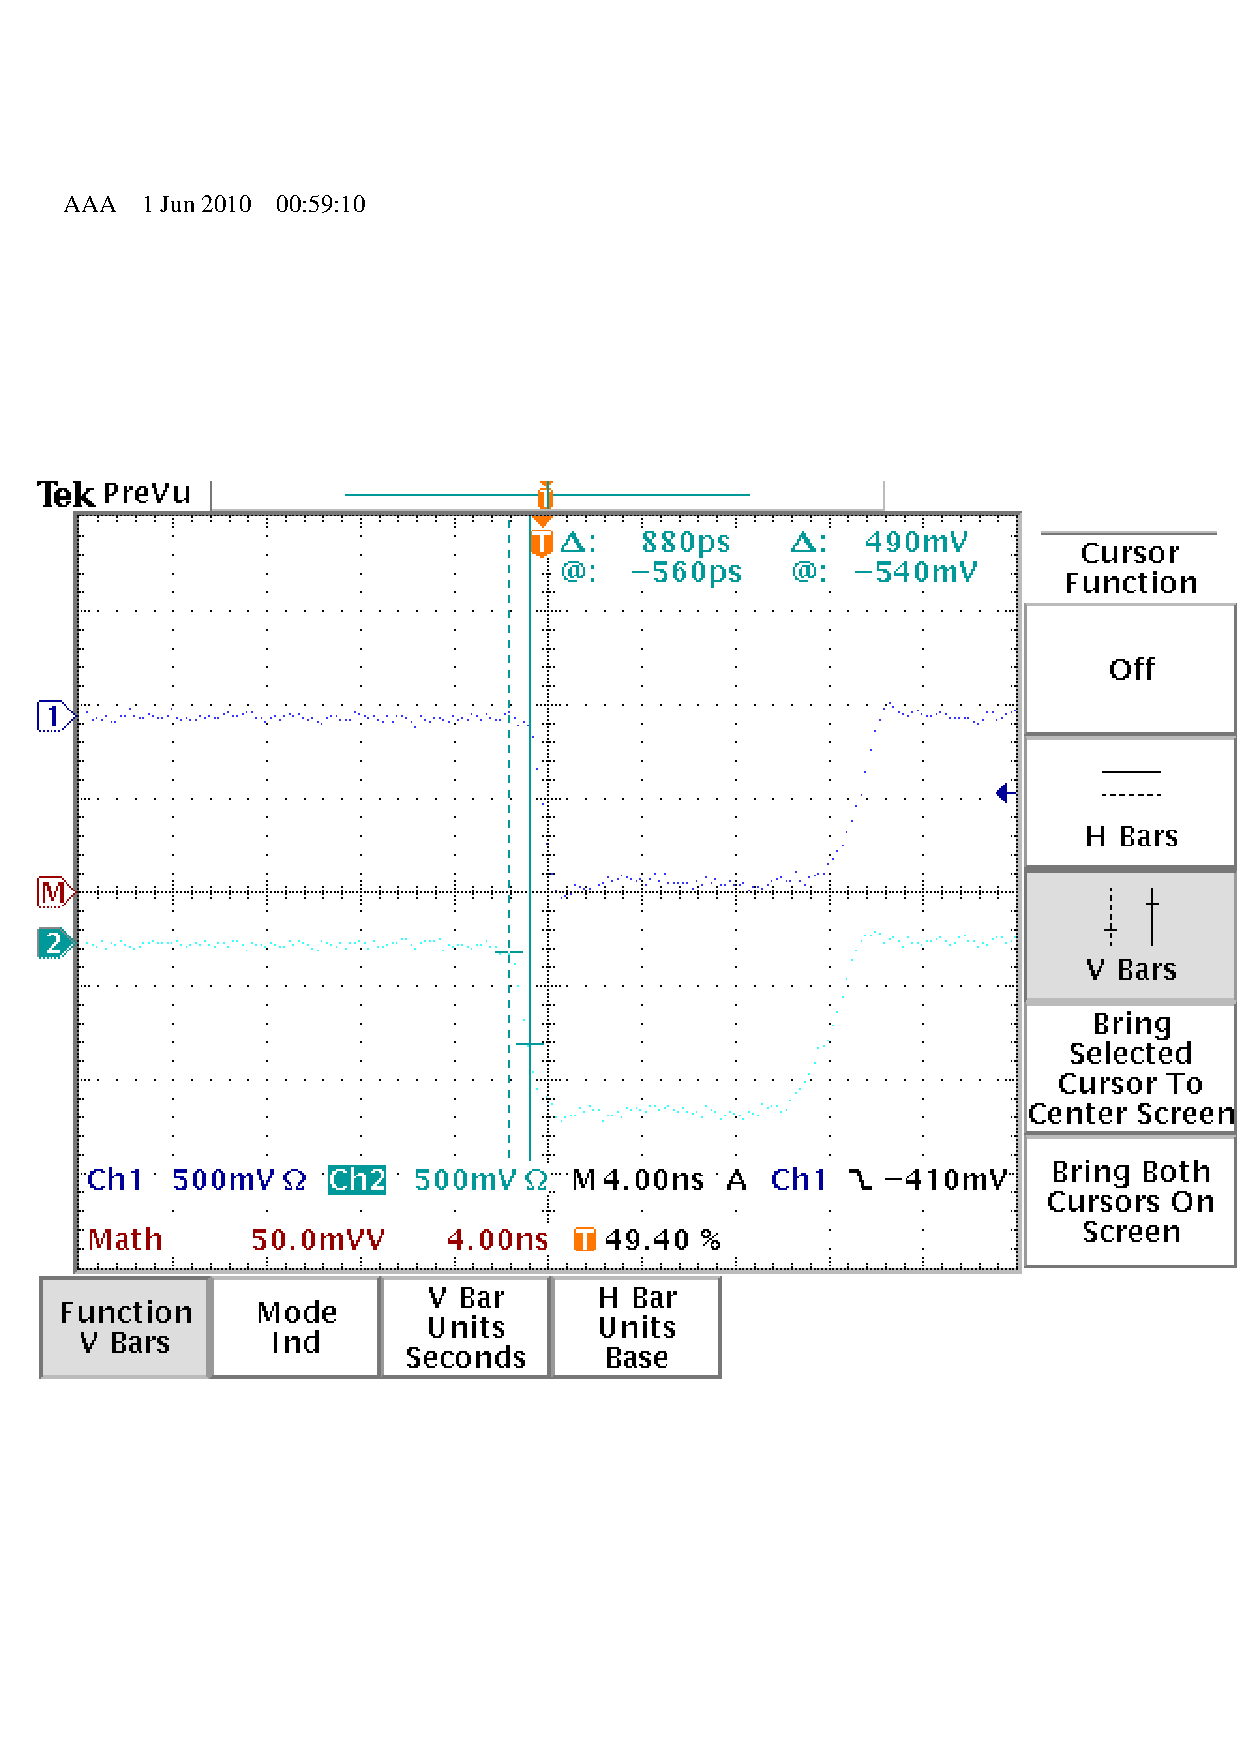
\includegraphics[width=0.375\textwidth,keepaspectratio,viewport=0 52 472 436,clip]{../tmp/TEK00006.pdf}}
  \subfloat[Zeitdifferenz 2]{
    \label{fig:zeitdiff_2}
    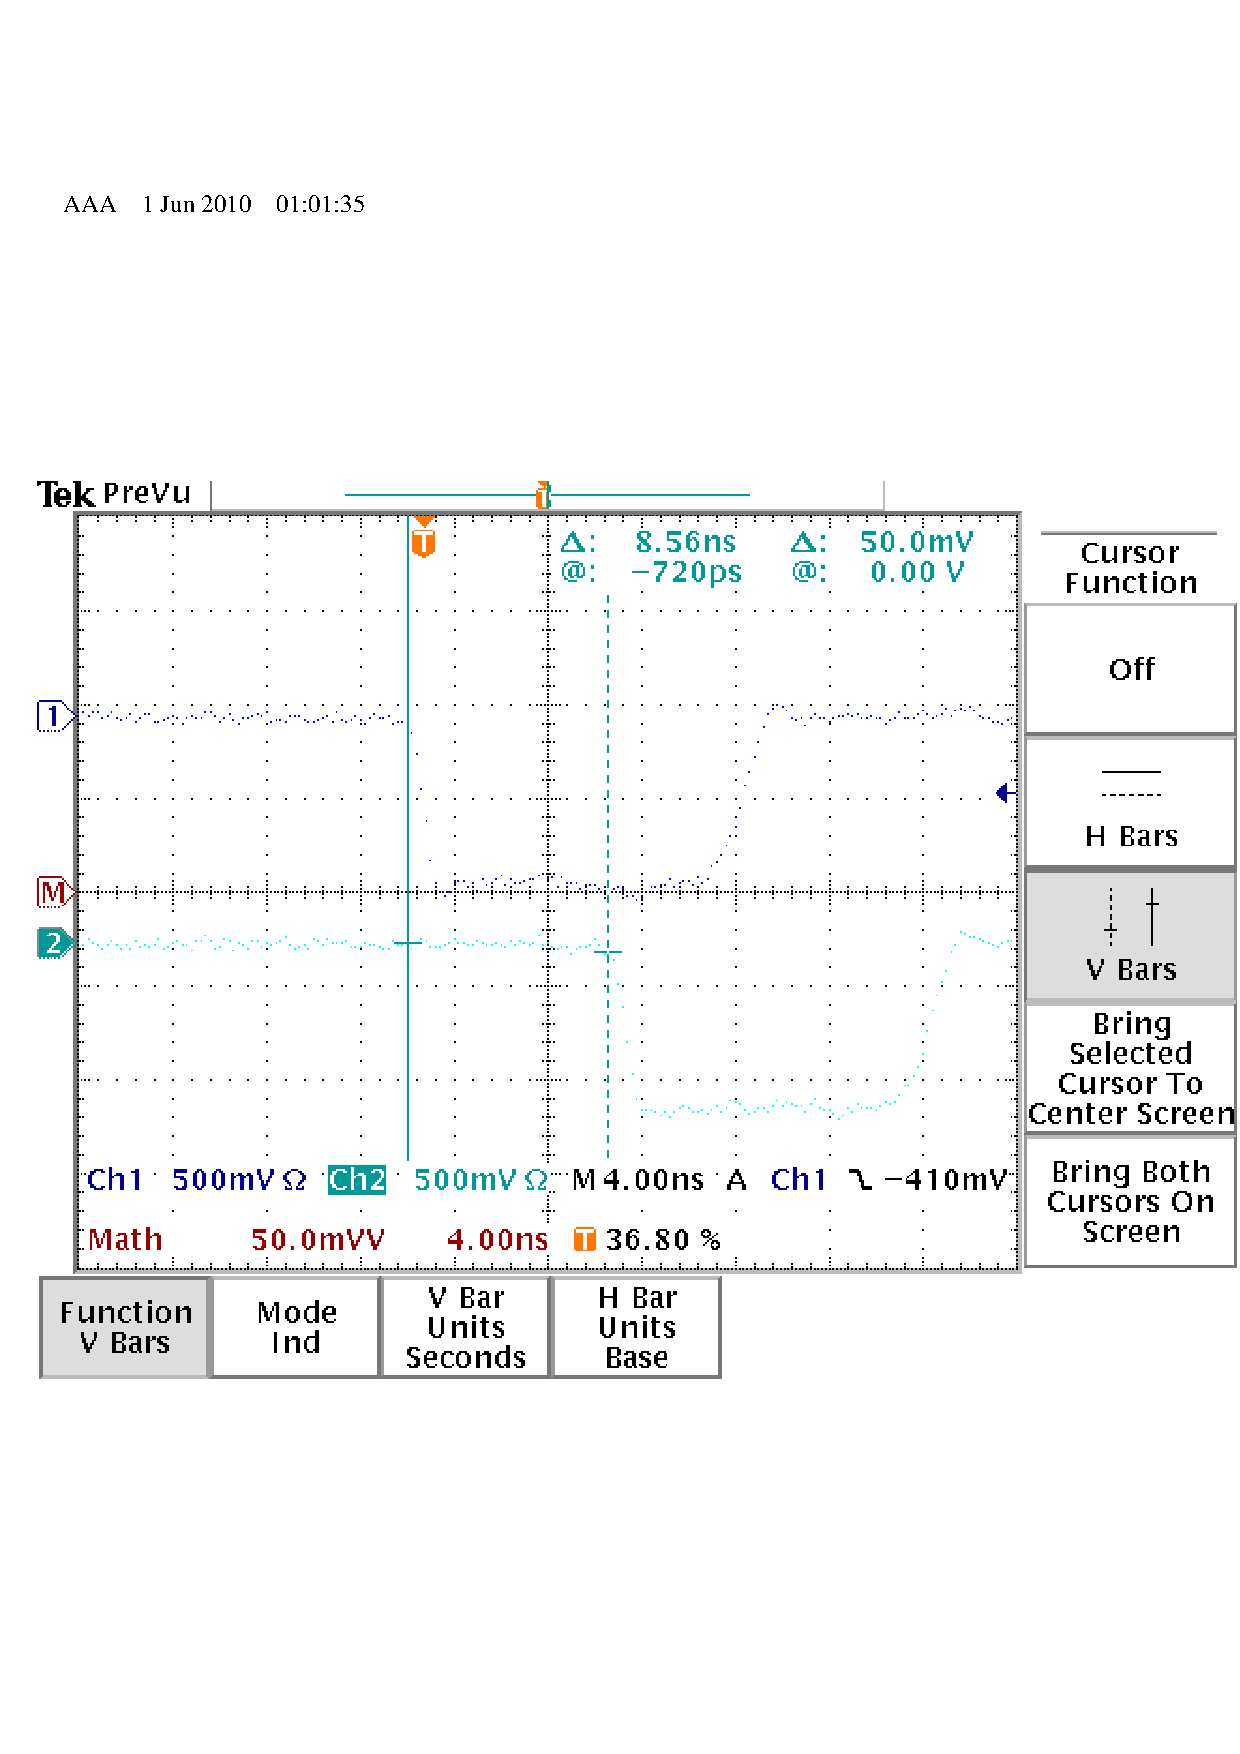
\includegraphics[width=0.375\textwidth,keepaspectratio,viewport=0 52 472 436,clip]{../tmp/TEK00007.pdf}
  }
  \newline
  \subfloat[Zeitdifferenz 3]{
    \label{fig:zeitdiff_3}
    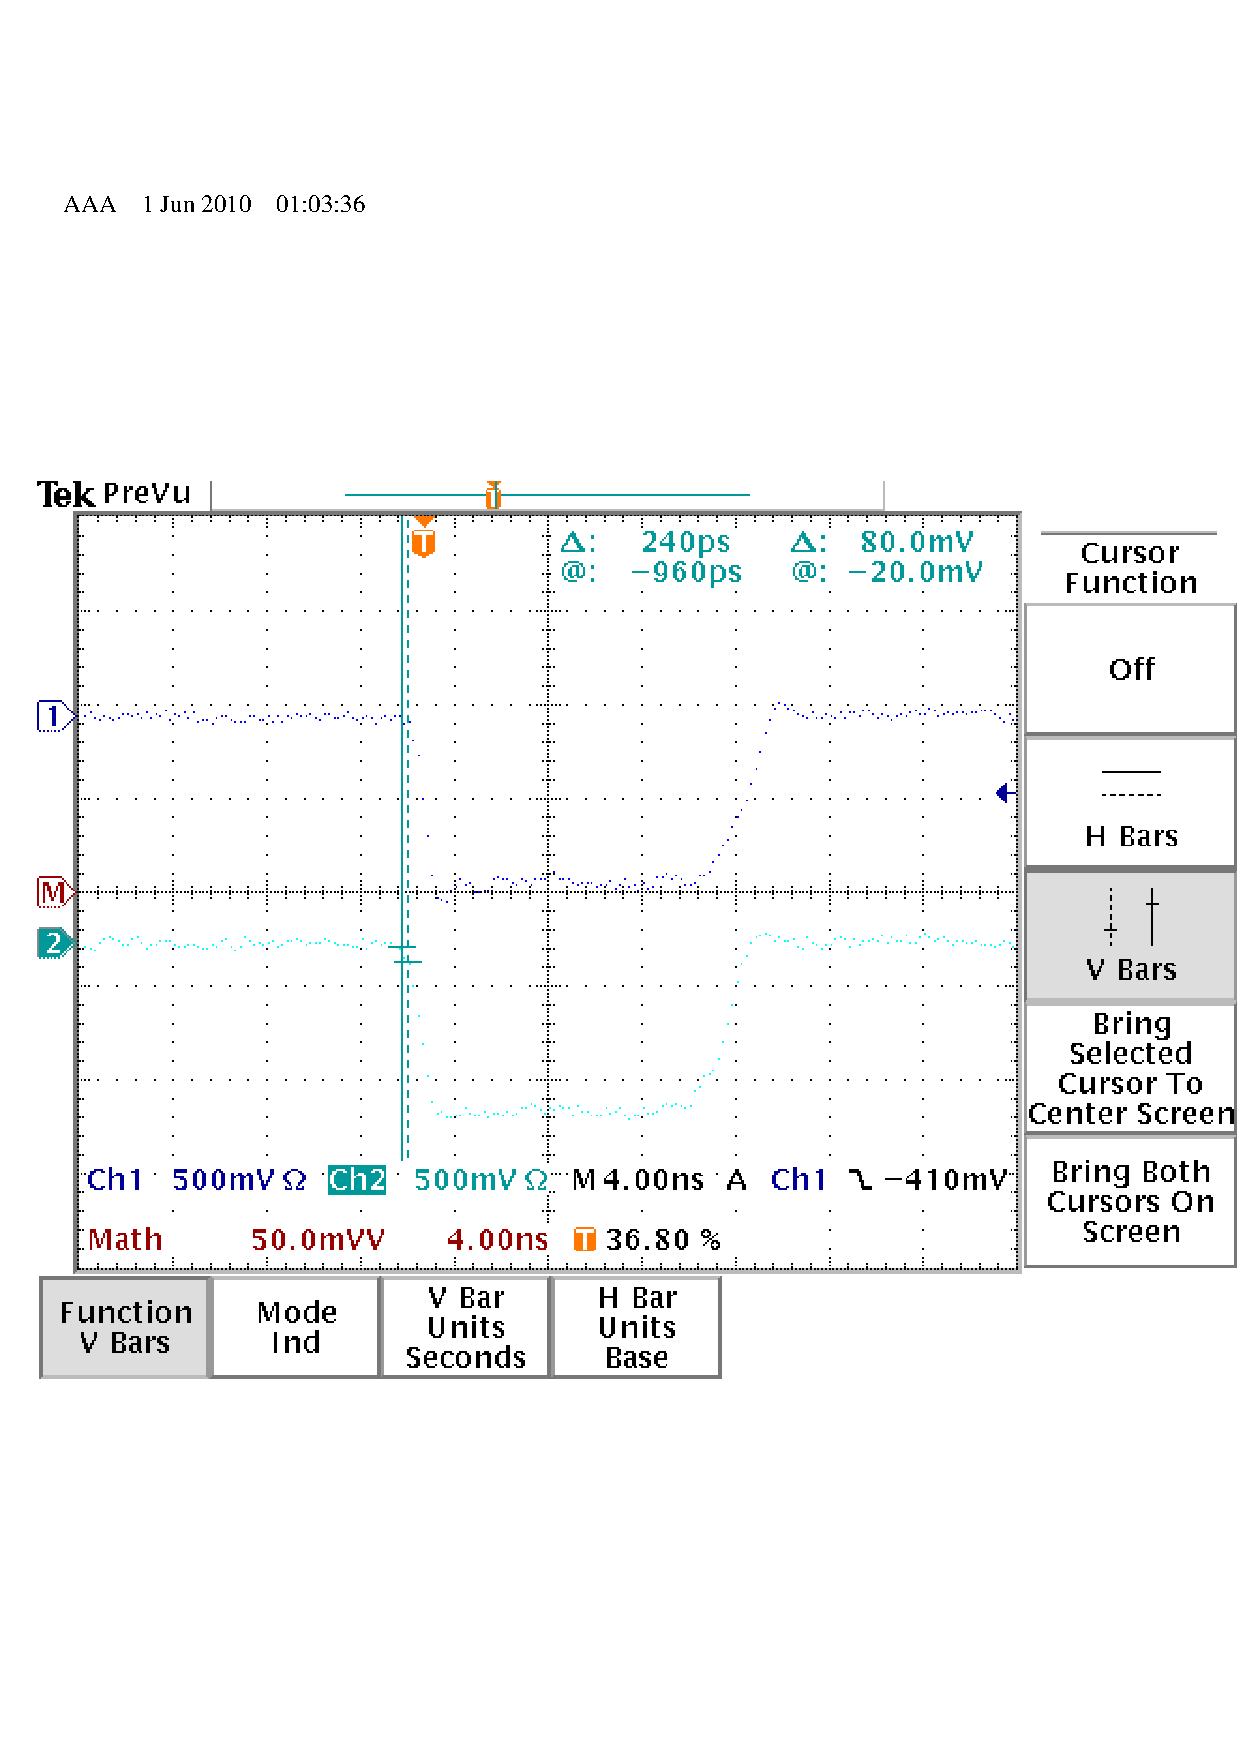
\includegraphics[width=0.375\textwidth,keepaspectratio,viewport=0 52 472 436,clip]{../tmp/TEK00008.pdf}
  }
  \subfloat[Zeitdifferenz 4]{
    \label{fig:zeitdiff_4}
    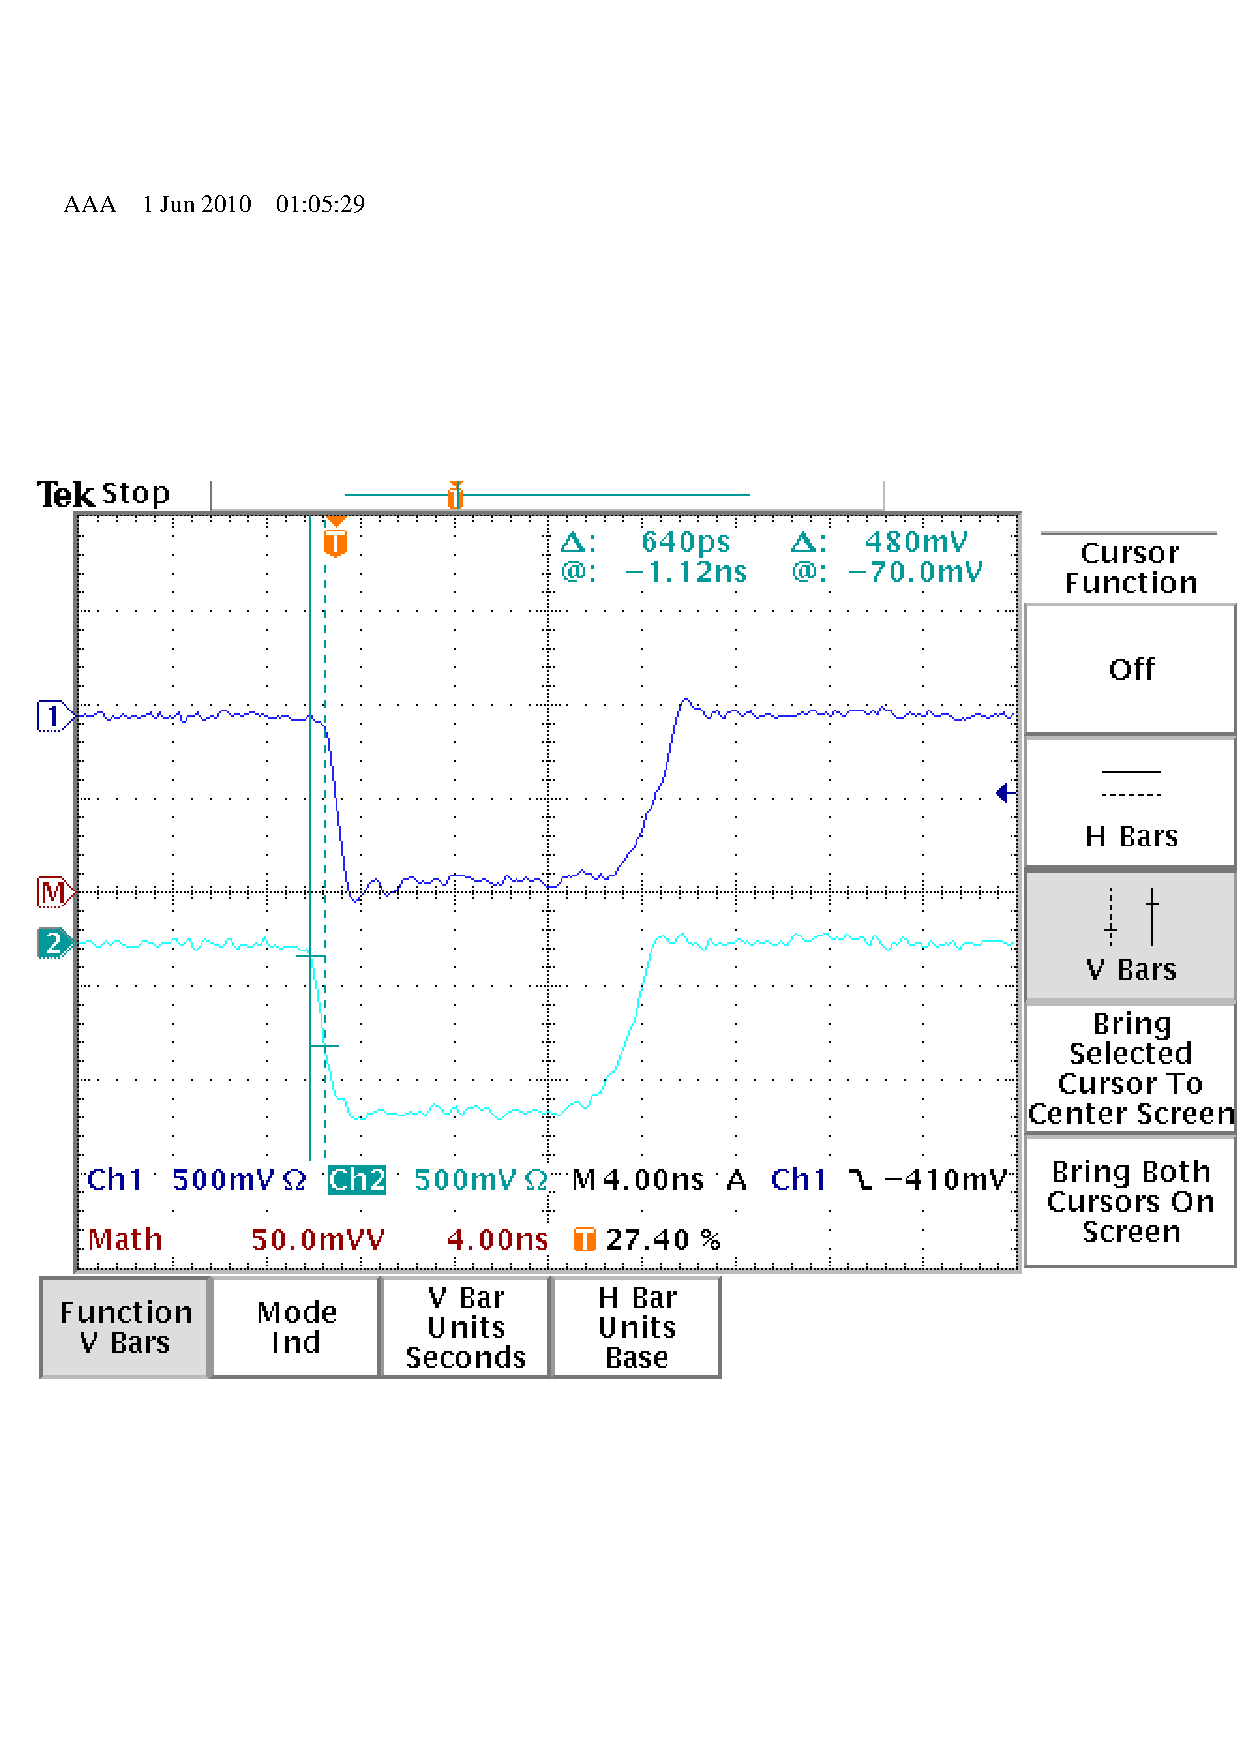
\includegraphics[width=0.375\textwidth,keepaspectratio,viewport=0 52 472 436,clip]{../tmp/TEK00009.pdf}
  }
  \newline
  \subfloat[Zeitdifferenz 5]{
    \label{fig:zeitdiff_5}
    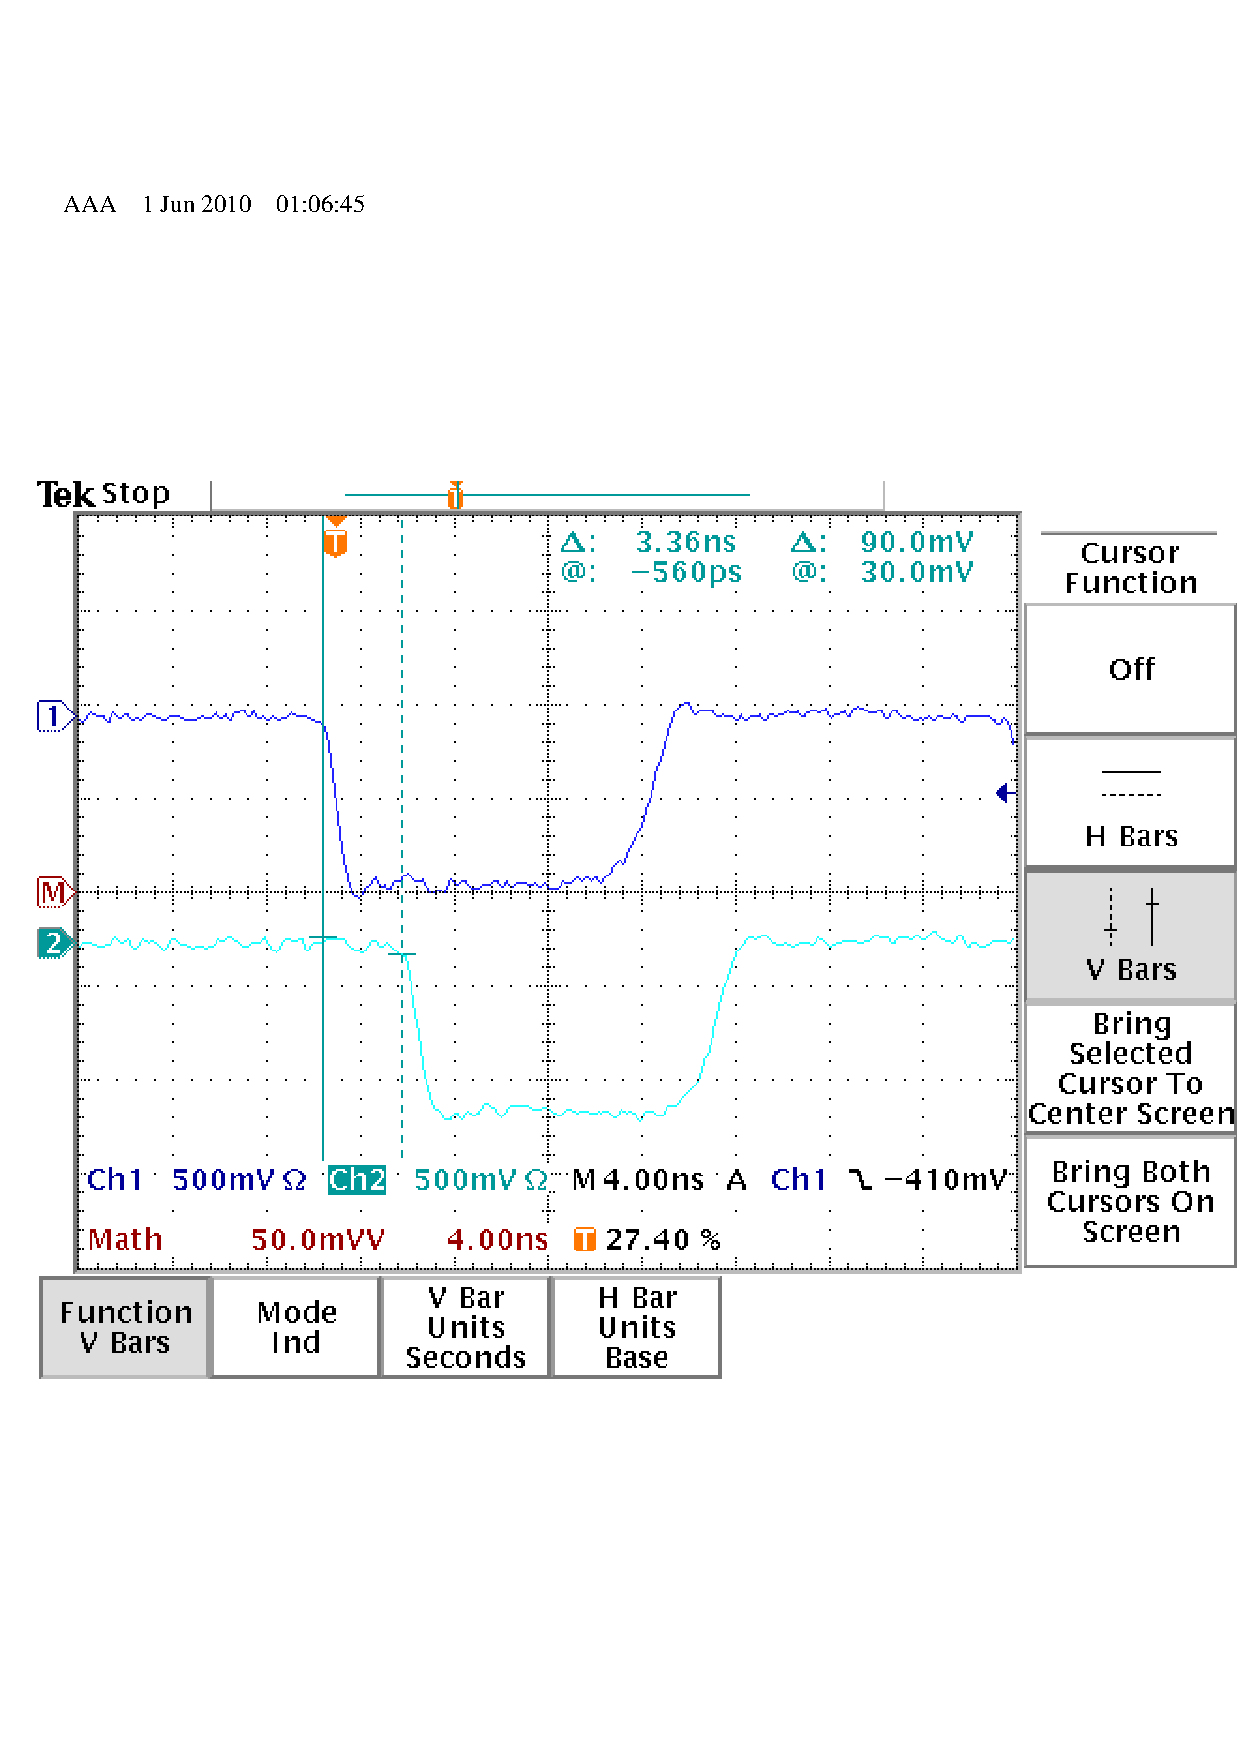
\includegraphics[width=0.375\textwidth,keepaspectratio,viewport=0 52 472 436,clip]{../tmp/TEK00010.pdf}
  }
  \subfloat[Zeitdifferenz 6]{
    \label{fig:zeitdiff_6}
    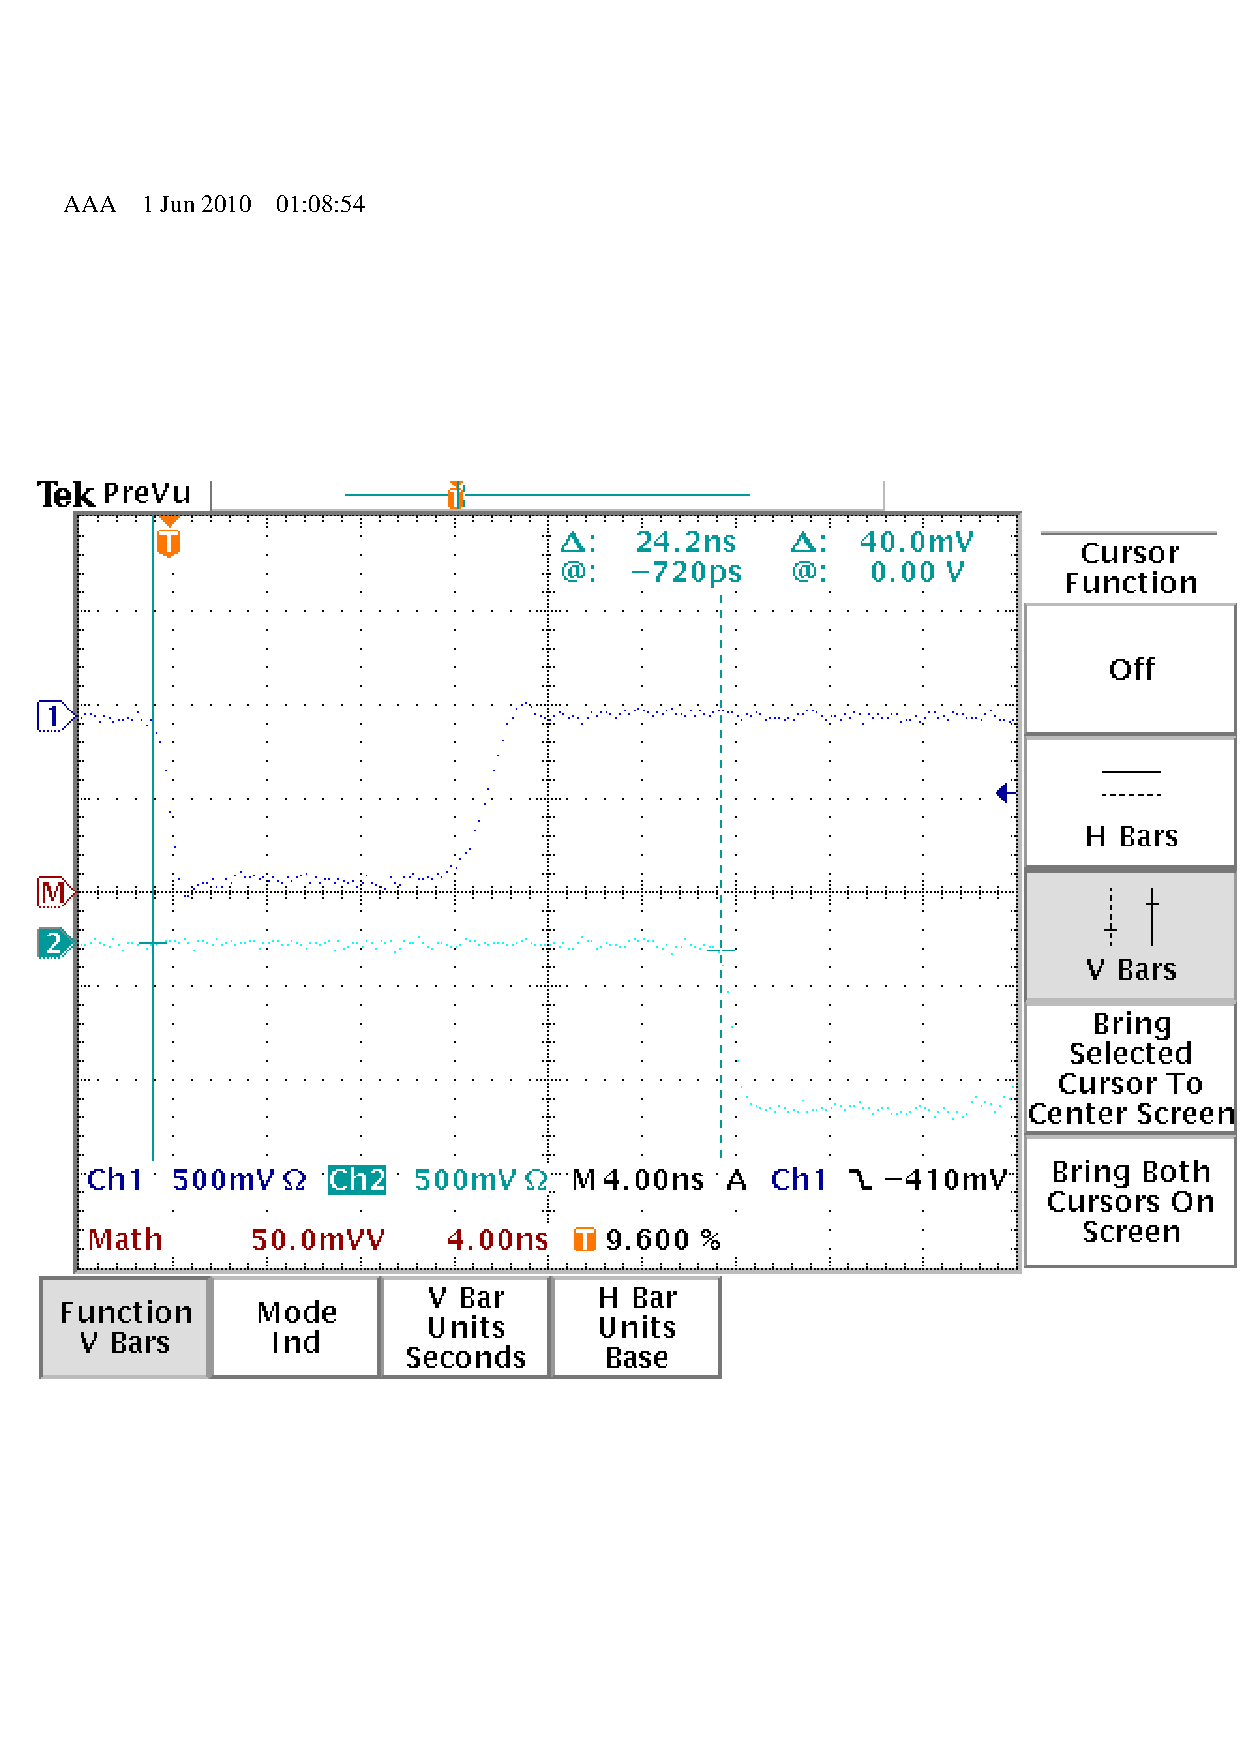
\includegraphics[width=0.375\textwidth,keepaspectratio,viewport=0 52 472 436,clip]{../tmp/TEK00011.pdf}
  }
  \newline
  \subfloat[Zeitdifferenz 7]{
    \label{fig:zeitdiff_7}
    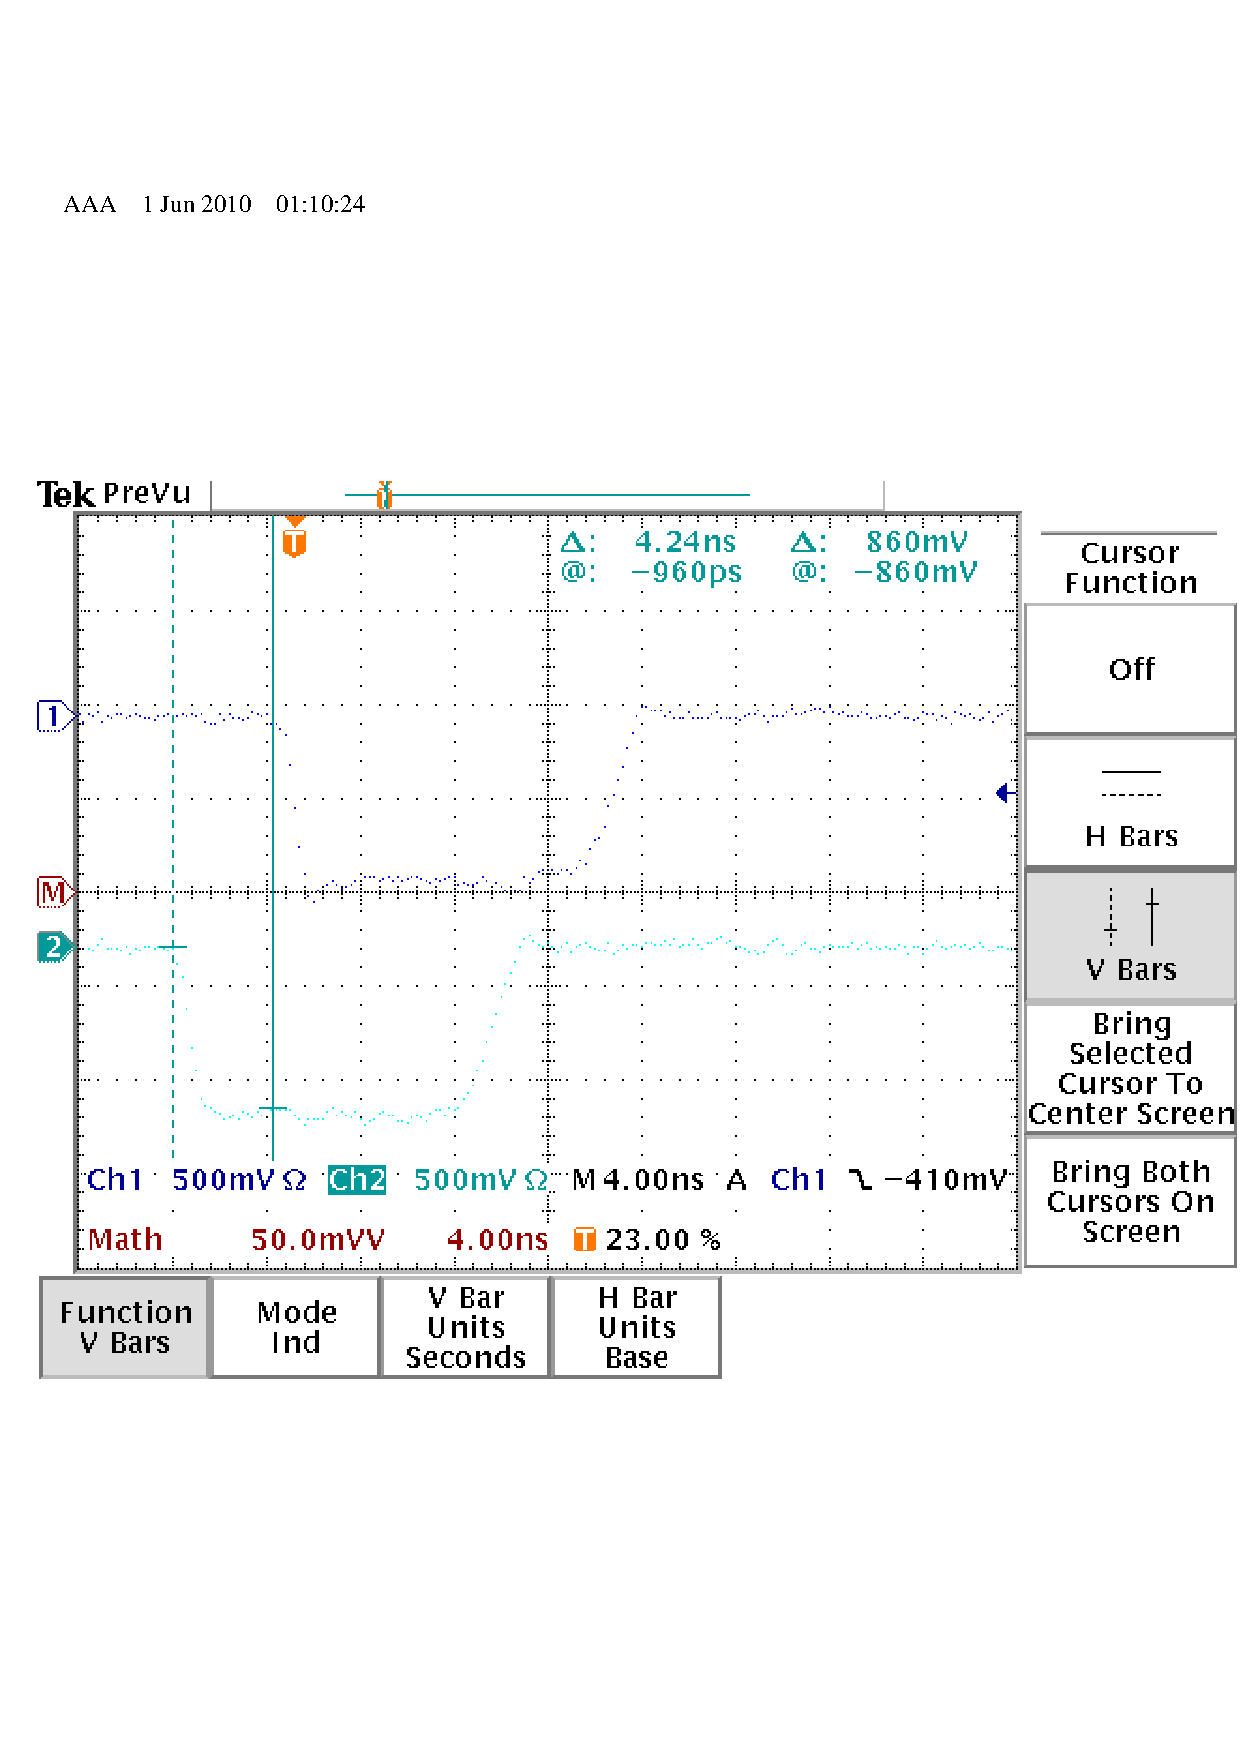
\includegraphics[width=0.375\textwidth,keepaspectratio,viewport=0 52 472 436,clip]{../tmp/TEK00012.pdf}
  }
  \caption{Zeitverzögerung zwischen den Photomultipliersignalen}
  \label{fig:zeitdifferenzen}
\end{center}
\end{figure}

\begin{figure}[htbp]
\begin{center}
  \subfloat[$SC_1 \wedge SC_2$, Ch1: $SC_1$, Ch2: $SC_2$, Trigger: UND-Schaltung]{
    \label{fig:sc1_und_sc2}
    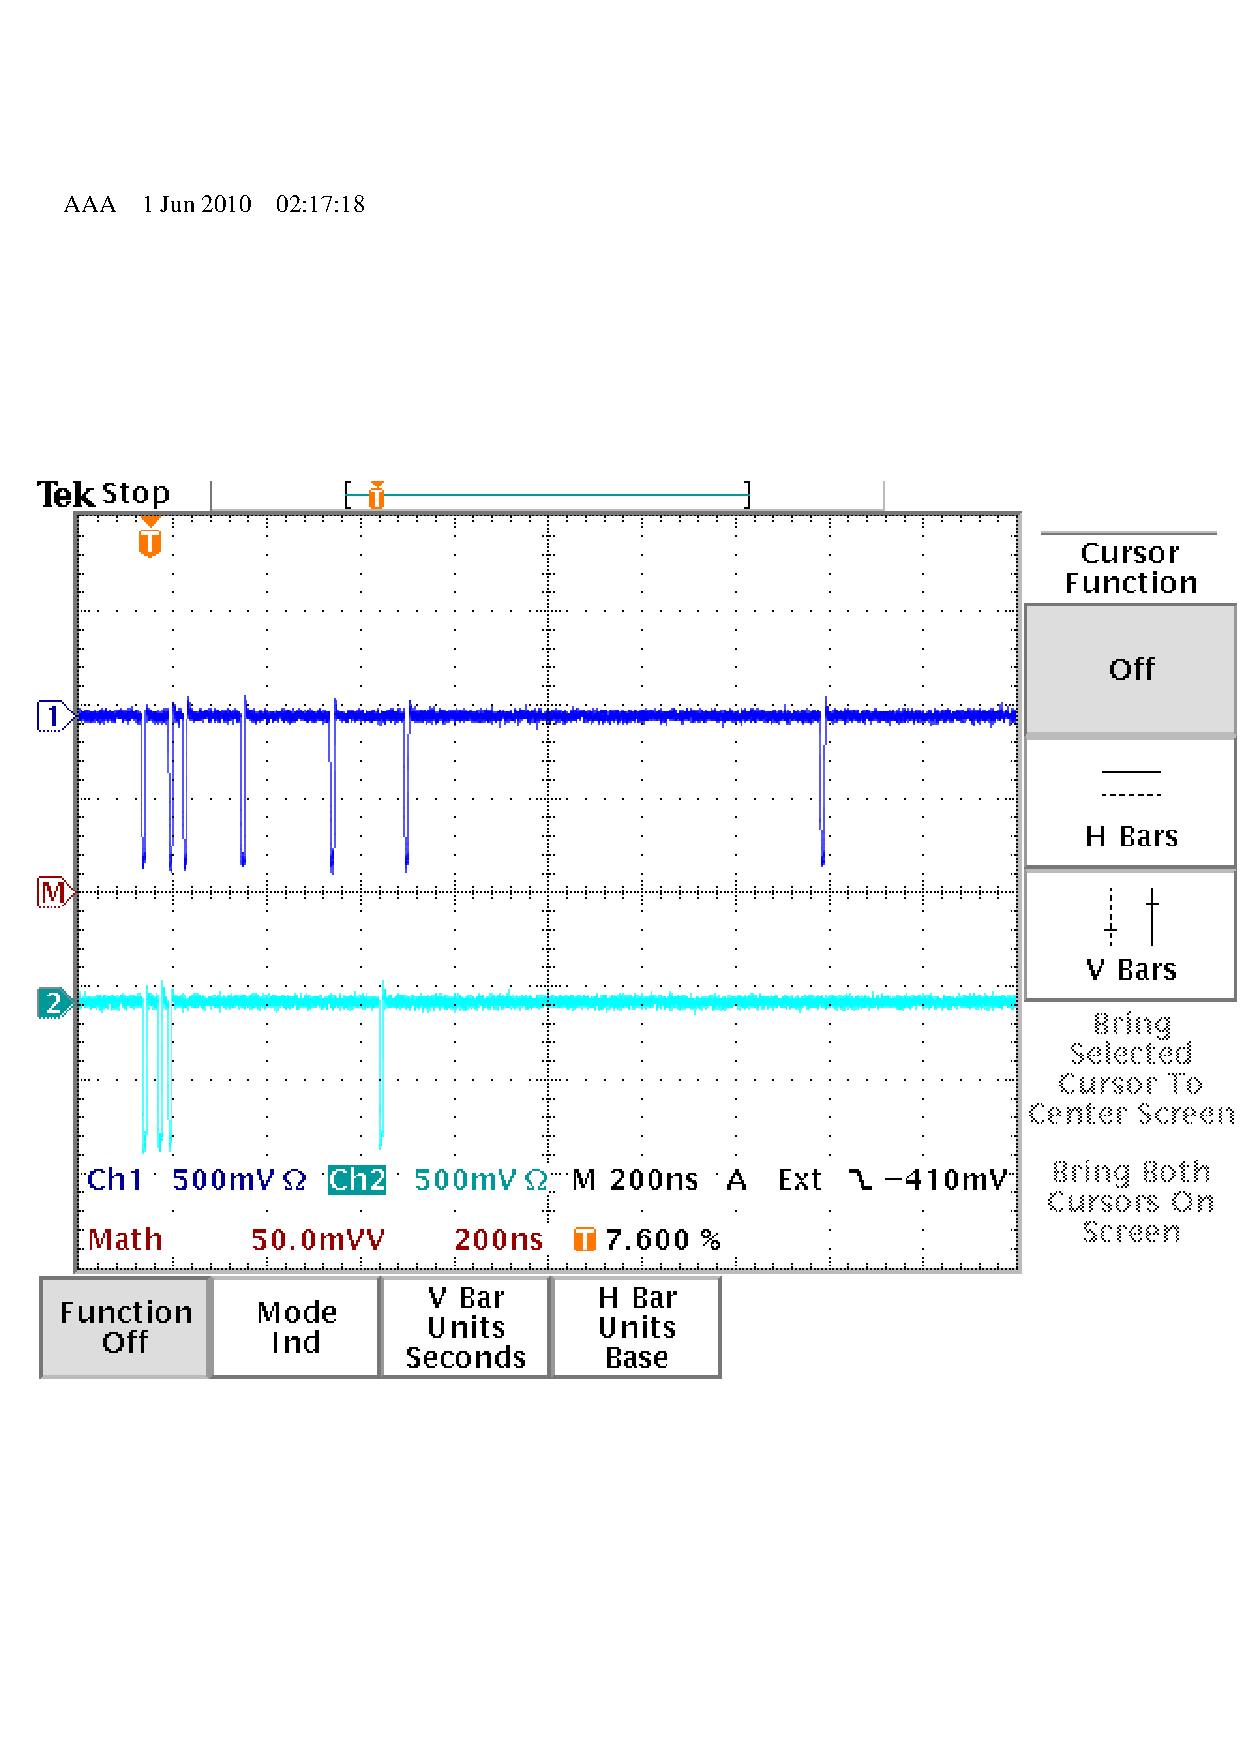
\includegraphics[width=0.45\textwidth,keepaspectratio,viewport=0 52 472 436,clip]{../tmp/TEK000019.pdf}
   }
  \subfloat[$SC_1 \wedge SC_2 \wedge SC_3$, Ch1: $SC_1$, Ch2: $SC_2 \wedge SC_3$, Trigger: UND-Schaltung]{
    \label{fig:sc1_und_sc2_und_sc3}
    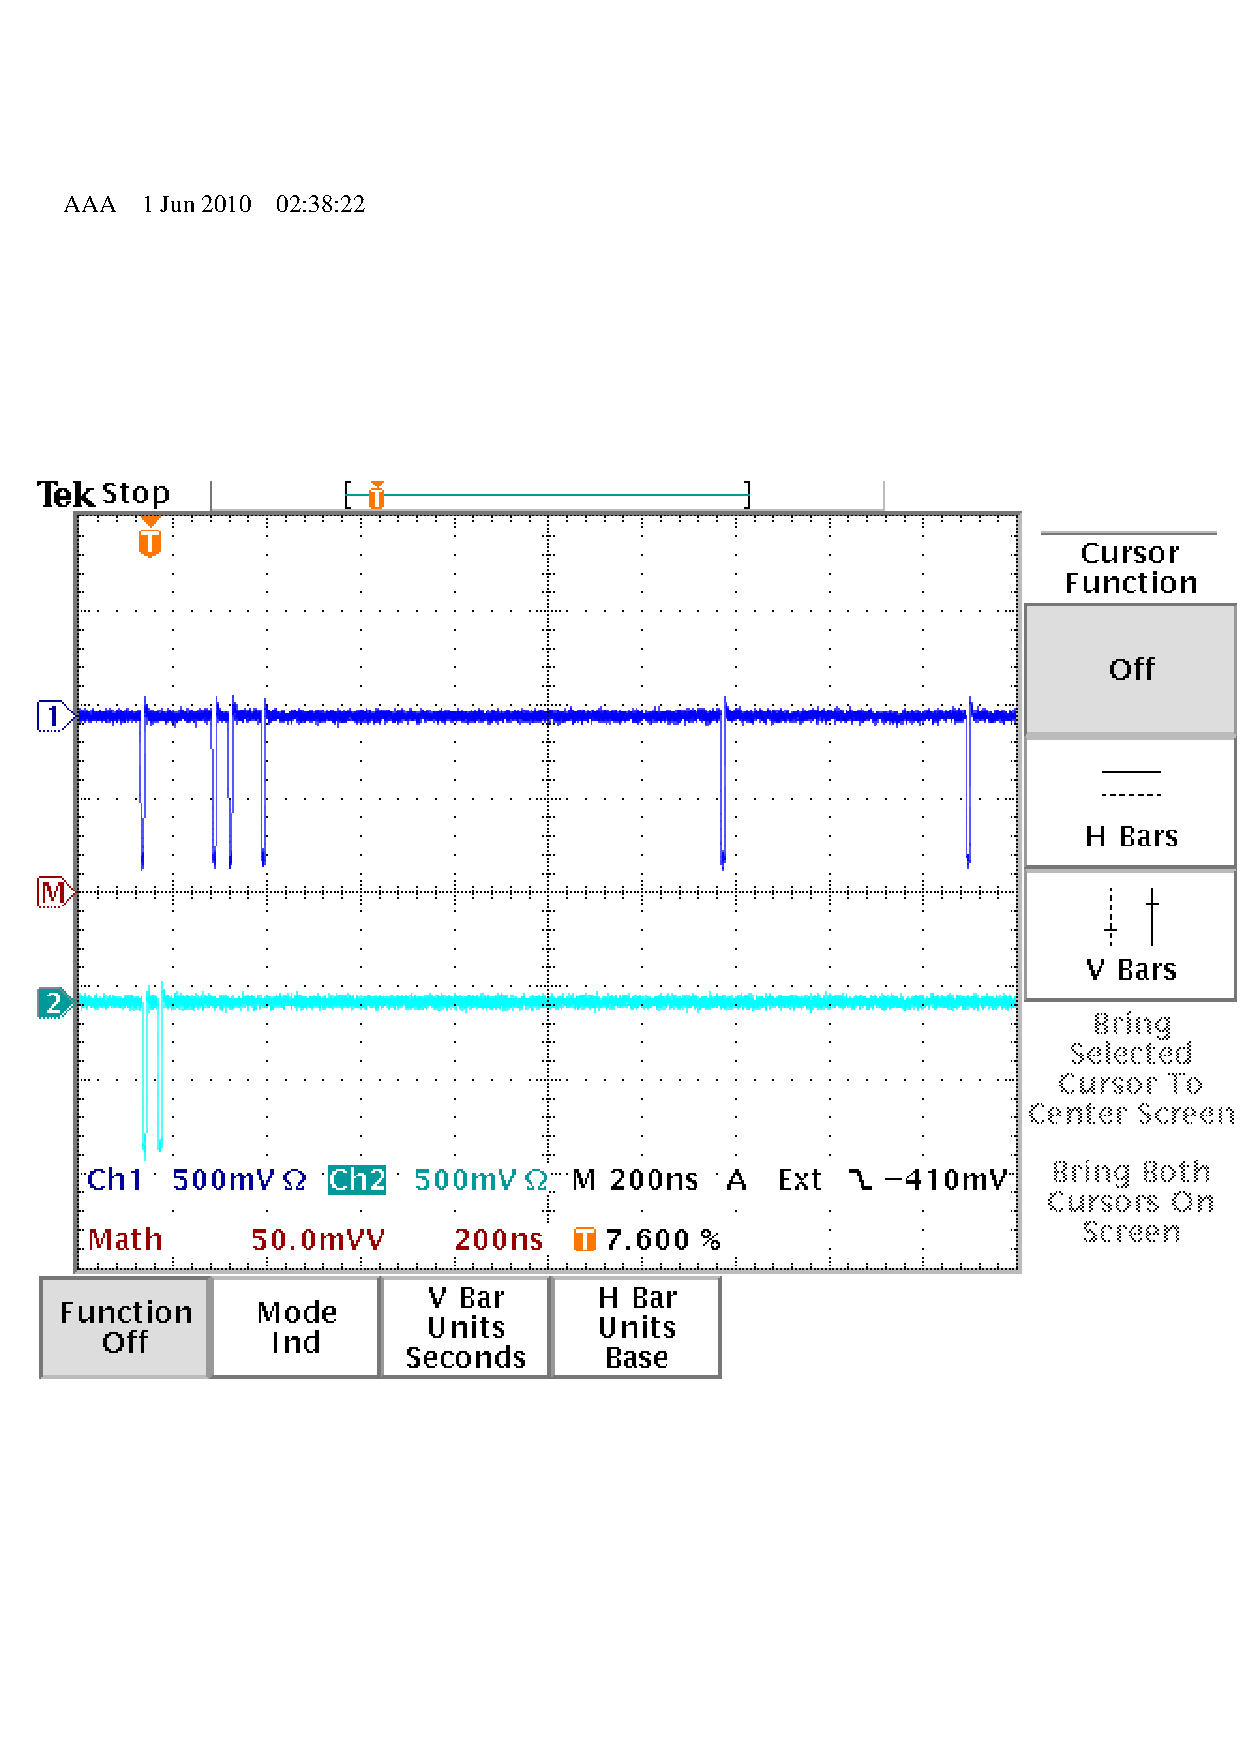
\includegraphics[width=0.45\textwidth,keepaspectratio,viewport=0 52 472 436,clip]{../tmp/TEK000021.pdf}
  }
  \newline
  \subfloat[Ch1: $SC_1 \wedge SC_2 \neg SC_3$, Trigger: Ch1]{
    \label{fig:sc1_und_sc2_not_sc3}
    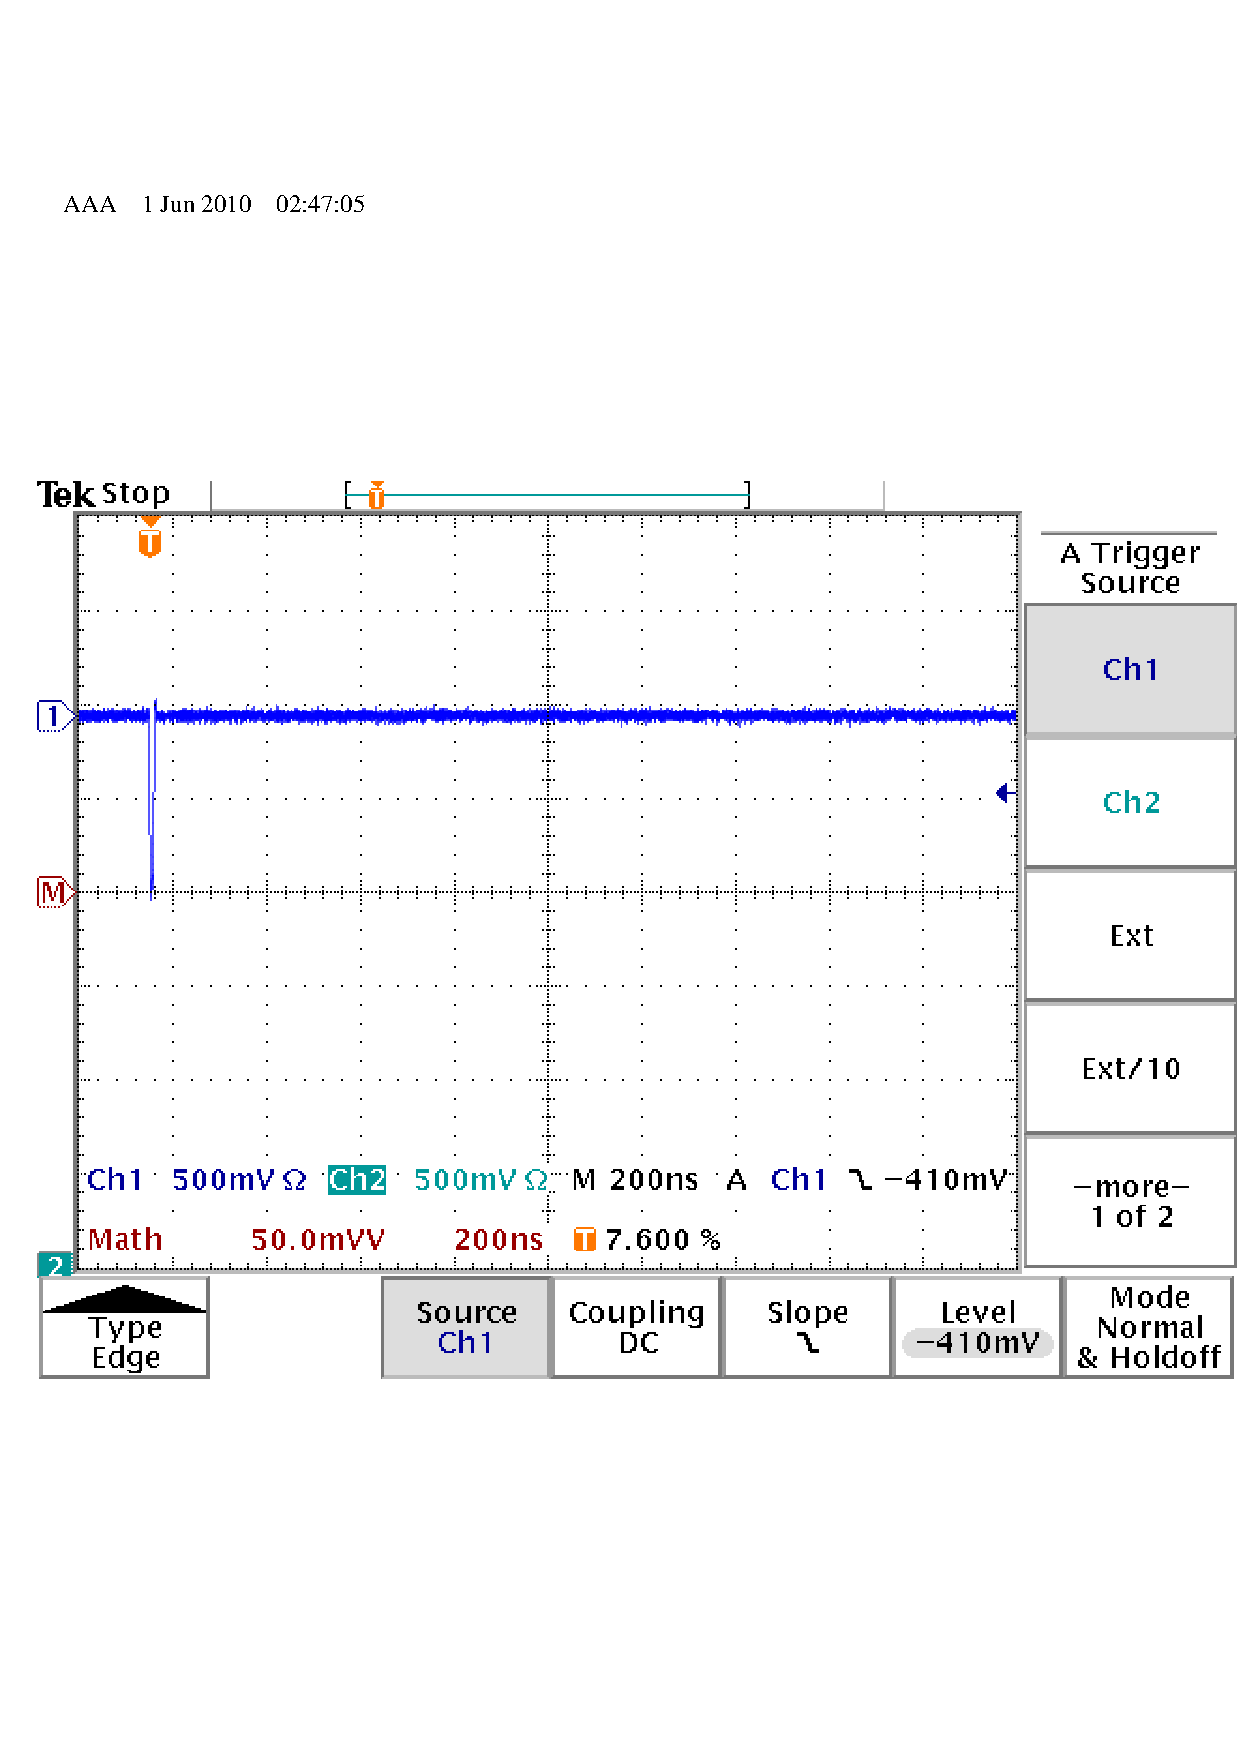
\includegraphics[width=0.45\textwidth,keepaspectratio,viewport=0 52 472 436,clip]{../tmp/TEK000022.pdf}
  }
  \subfloat[Ch1: $SC_2 \wedge SC_3$, Trigger: Ch1]{
    \label{fig:sc2_und_sc3}
    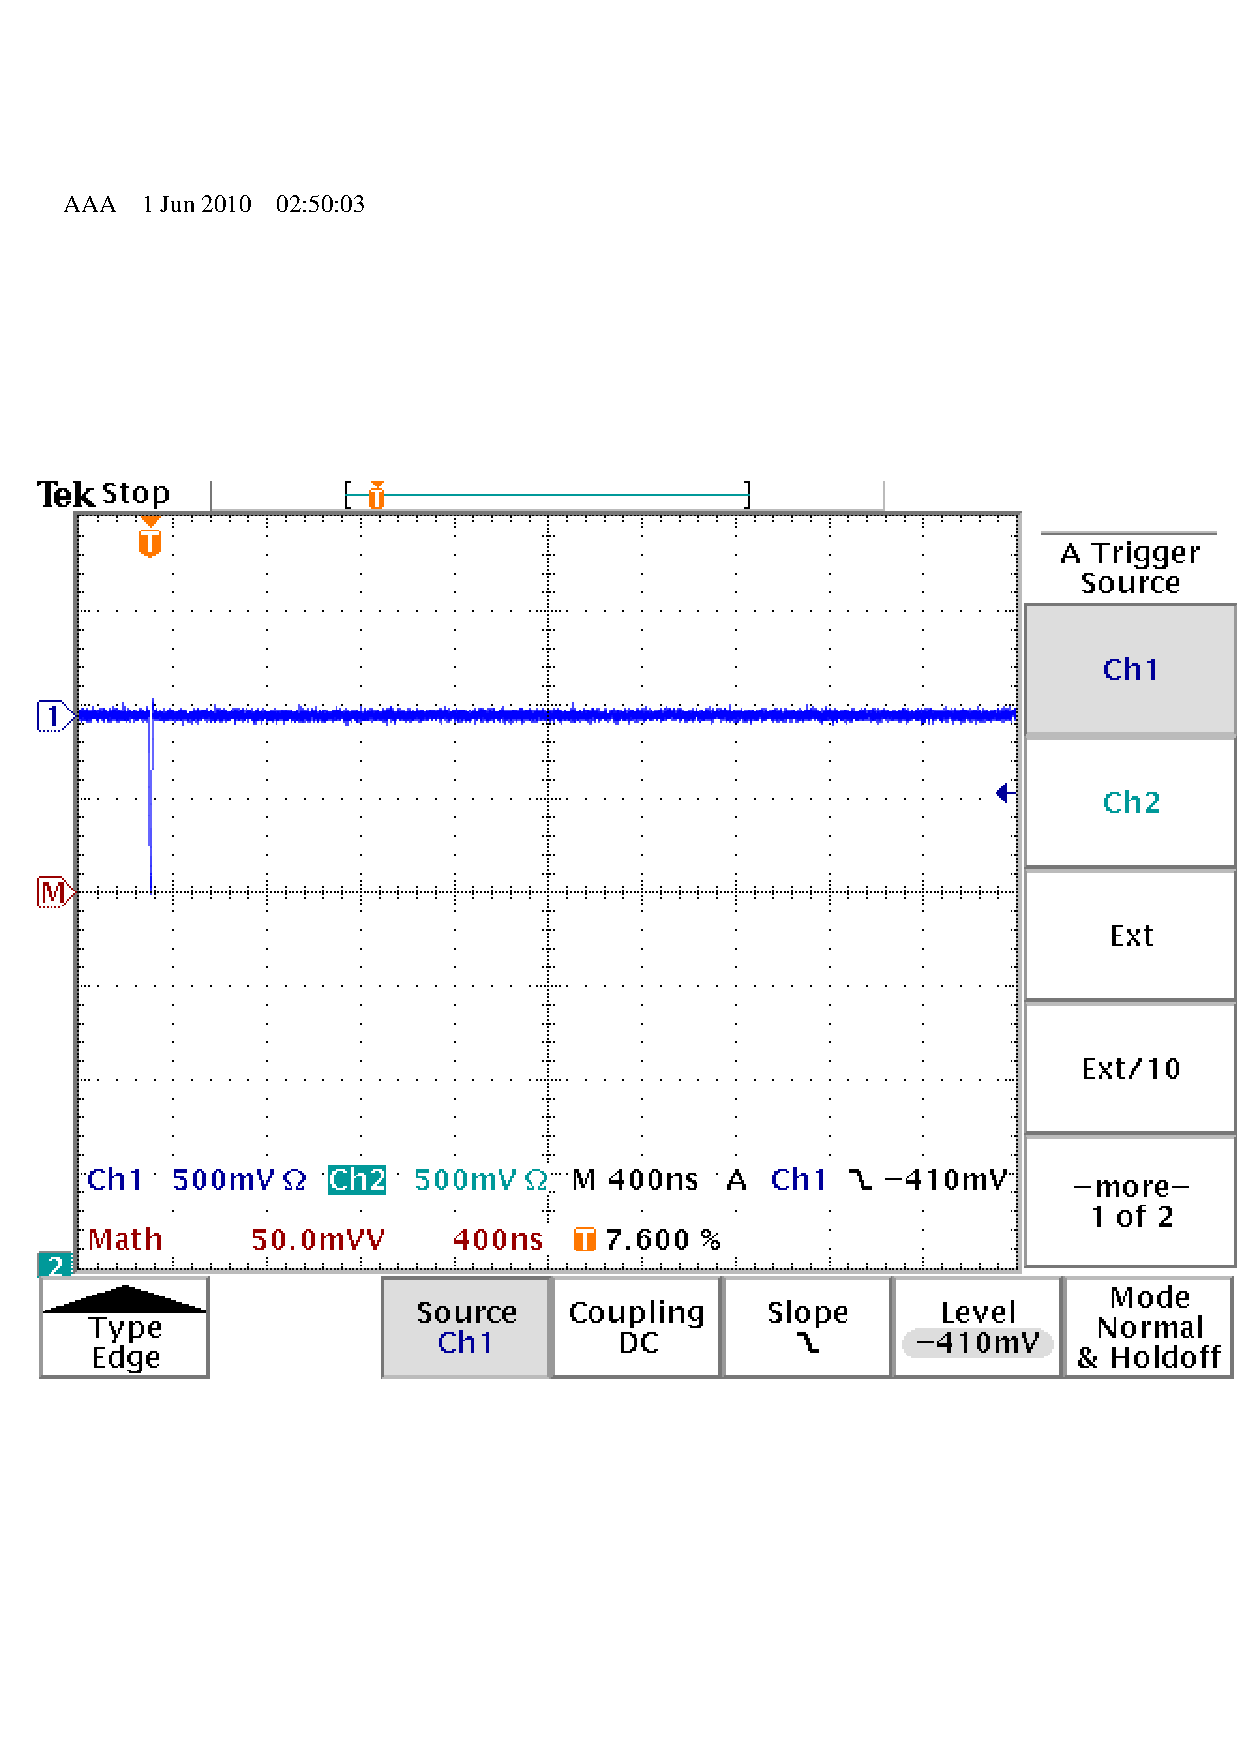
\includegraphics[width=0.45\textwidth,keepaspectratio,viewport=0 52 472 436,clip]{../tmp/TEK000023.pdf}
  }
  \newline
  \subfloat[$SC_2 \vee SC_3$, Ch1: $SC_2$, Ch2: $SC_3$, Trigger: UND-Signal]{
    \label{fig:sc2_oder_sc3}
    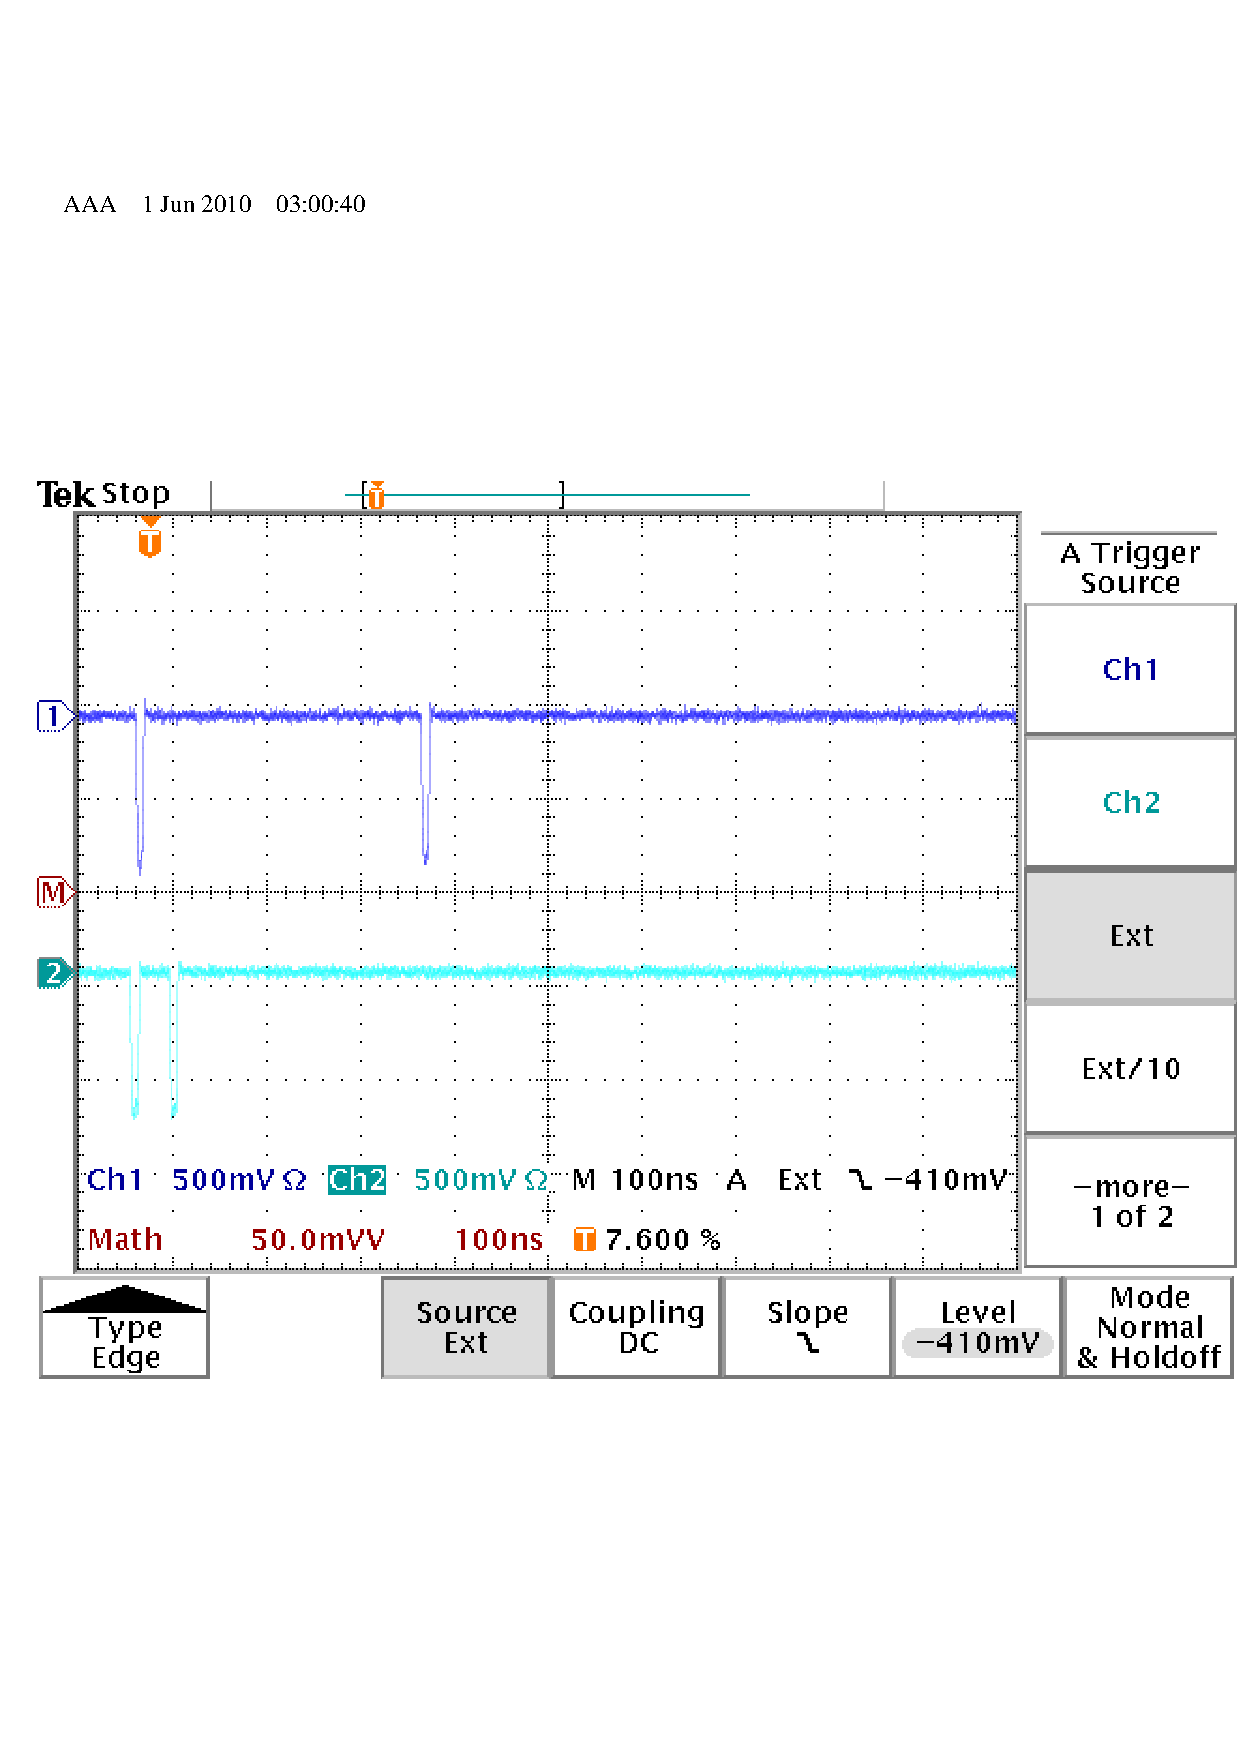
\includegraphics[width=0.45\textwidth,keepaspectratio,viewport=0 52 472 436,clip]{../tmp/TEK000025.pdf}
  }
  \caption{Signale bei verschiedenen Kombinationen von Szintillationszählern}
  \label{fig:kombinationen}
\end{center}
\end{figure}

\begin{figure}[htbp]
\begin{center}
  \subfloat[$SC_1 \neg SC_2 \neg SC_3$, Ch1: NOT-Signal, Ch2: $SC_1$, Trigger: Ch1]{
    \label{fig:nur_sc1}
    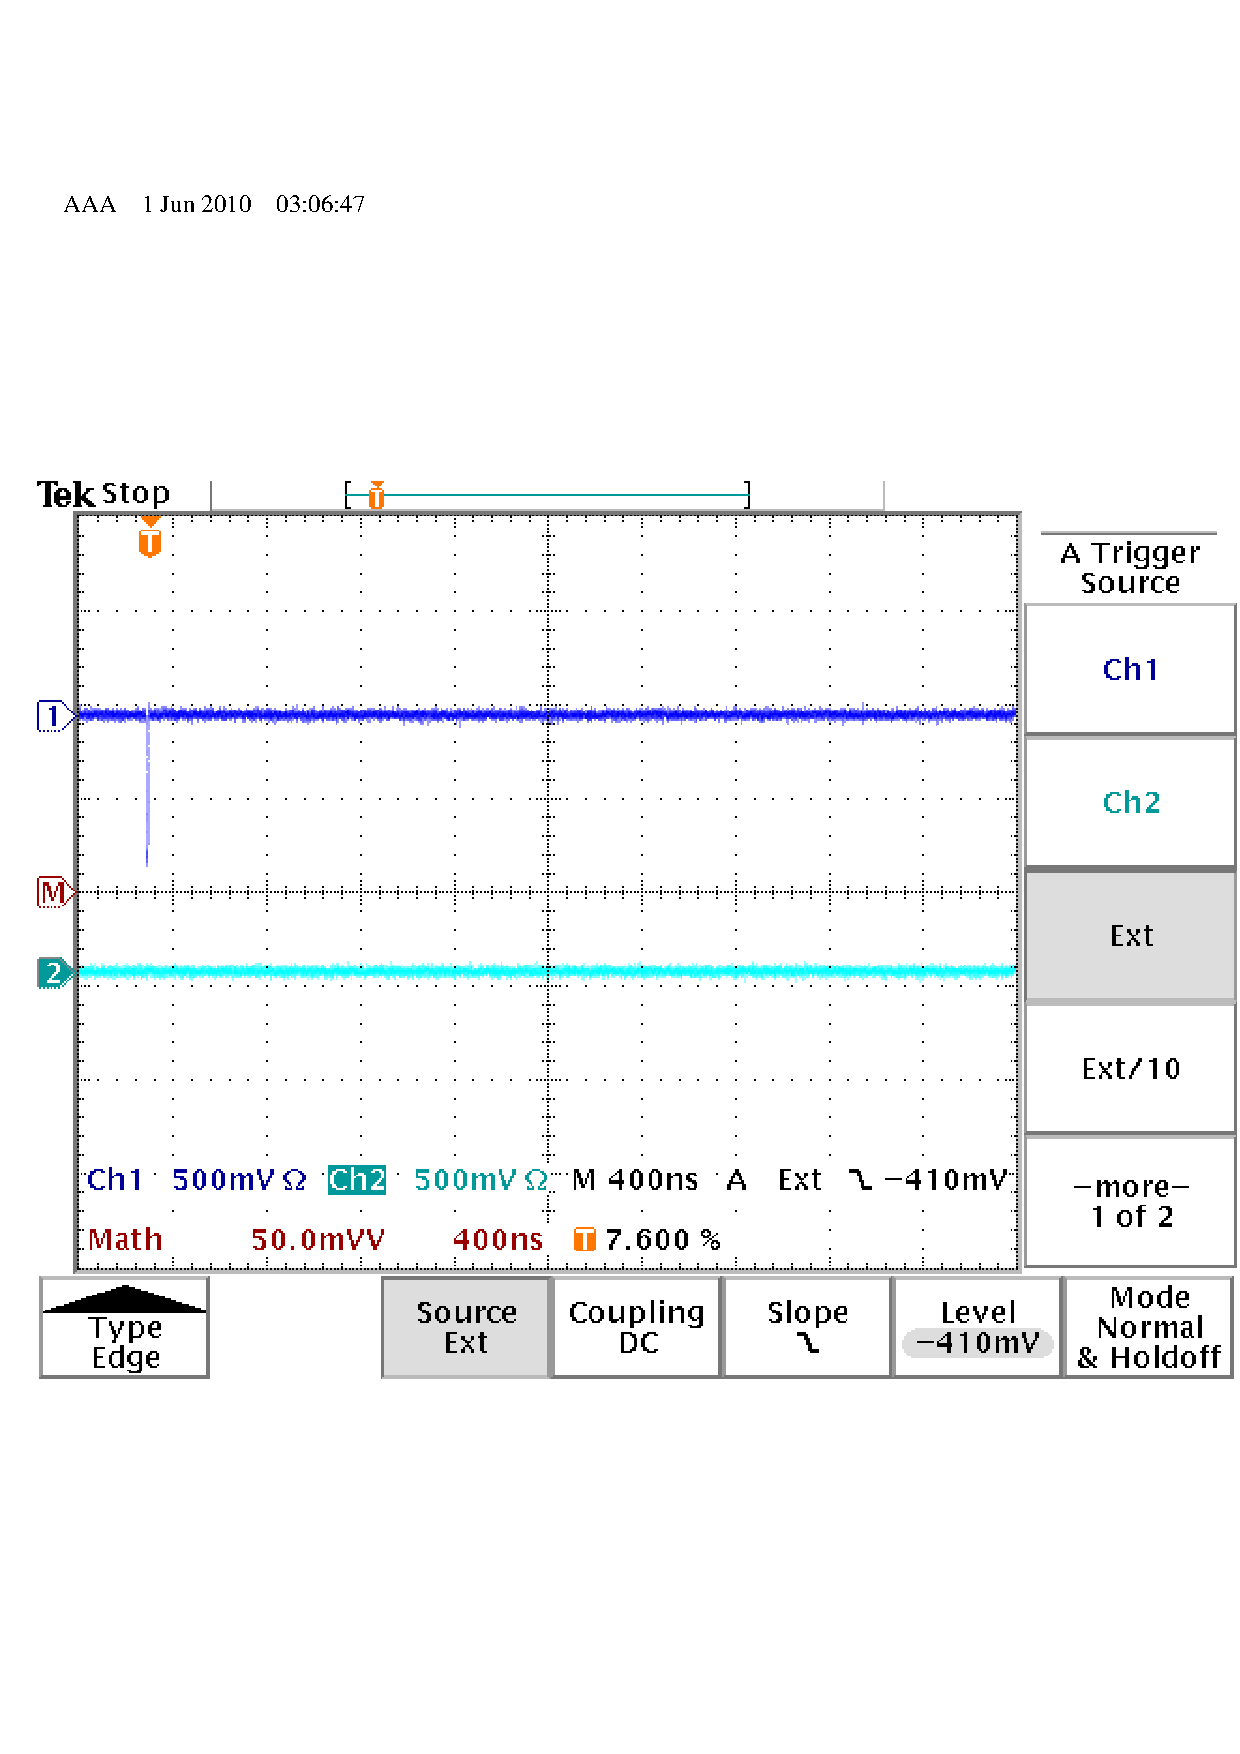
\includegraphics[width=0.45\textwidth,keepaspectratio,viewport=0 52 472 436,clip]{../tmp/TEK000026.pdf}
   }
  \subfloat[$\neg SC_1 \wedge SC_2 \neg SC_3$, Ch1: NOT-Signal, Ch2: $SC_2$, Trigger: Ch1]{
    \label{fig:nur_sc2}
    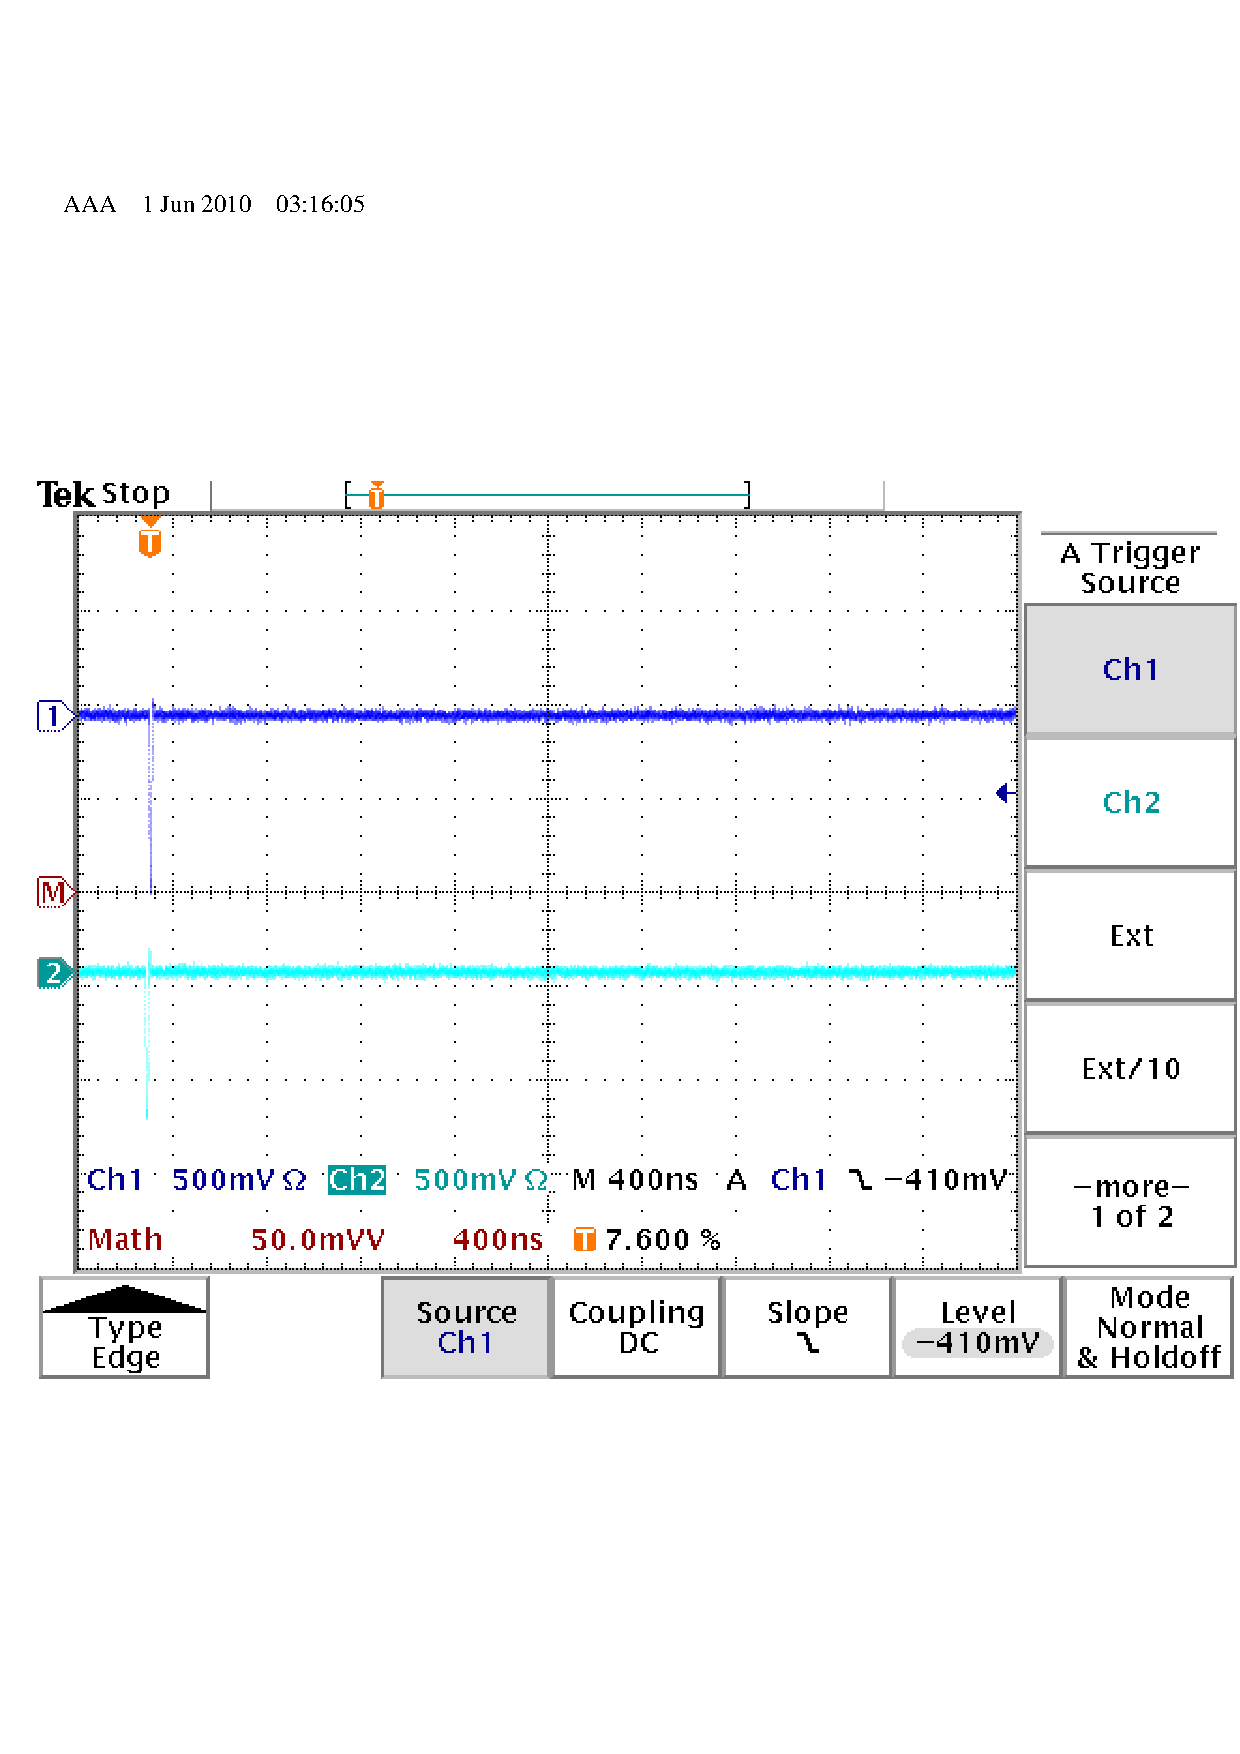
\includegraphics[width=0.45\textwidth,keepaspectratio,viewport=0 52 472 436,clip]{../tmp/TEK000027.pdf}
  }
  \newline
  \subfloat[$\neg SC_1 \neg SC_2 \wedge SC_3$, Ch1: NOT-Signal, Ch2: $SC_3$, Trigger: Ch1]{
    \label{fig:nur_sc3}
    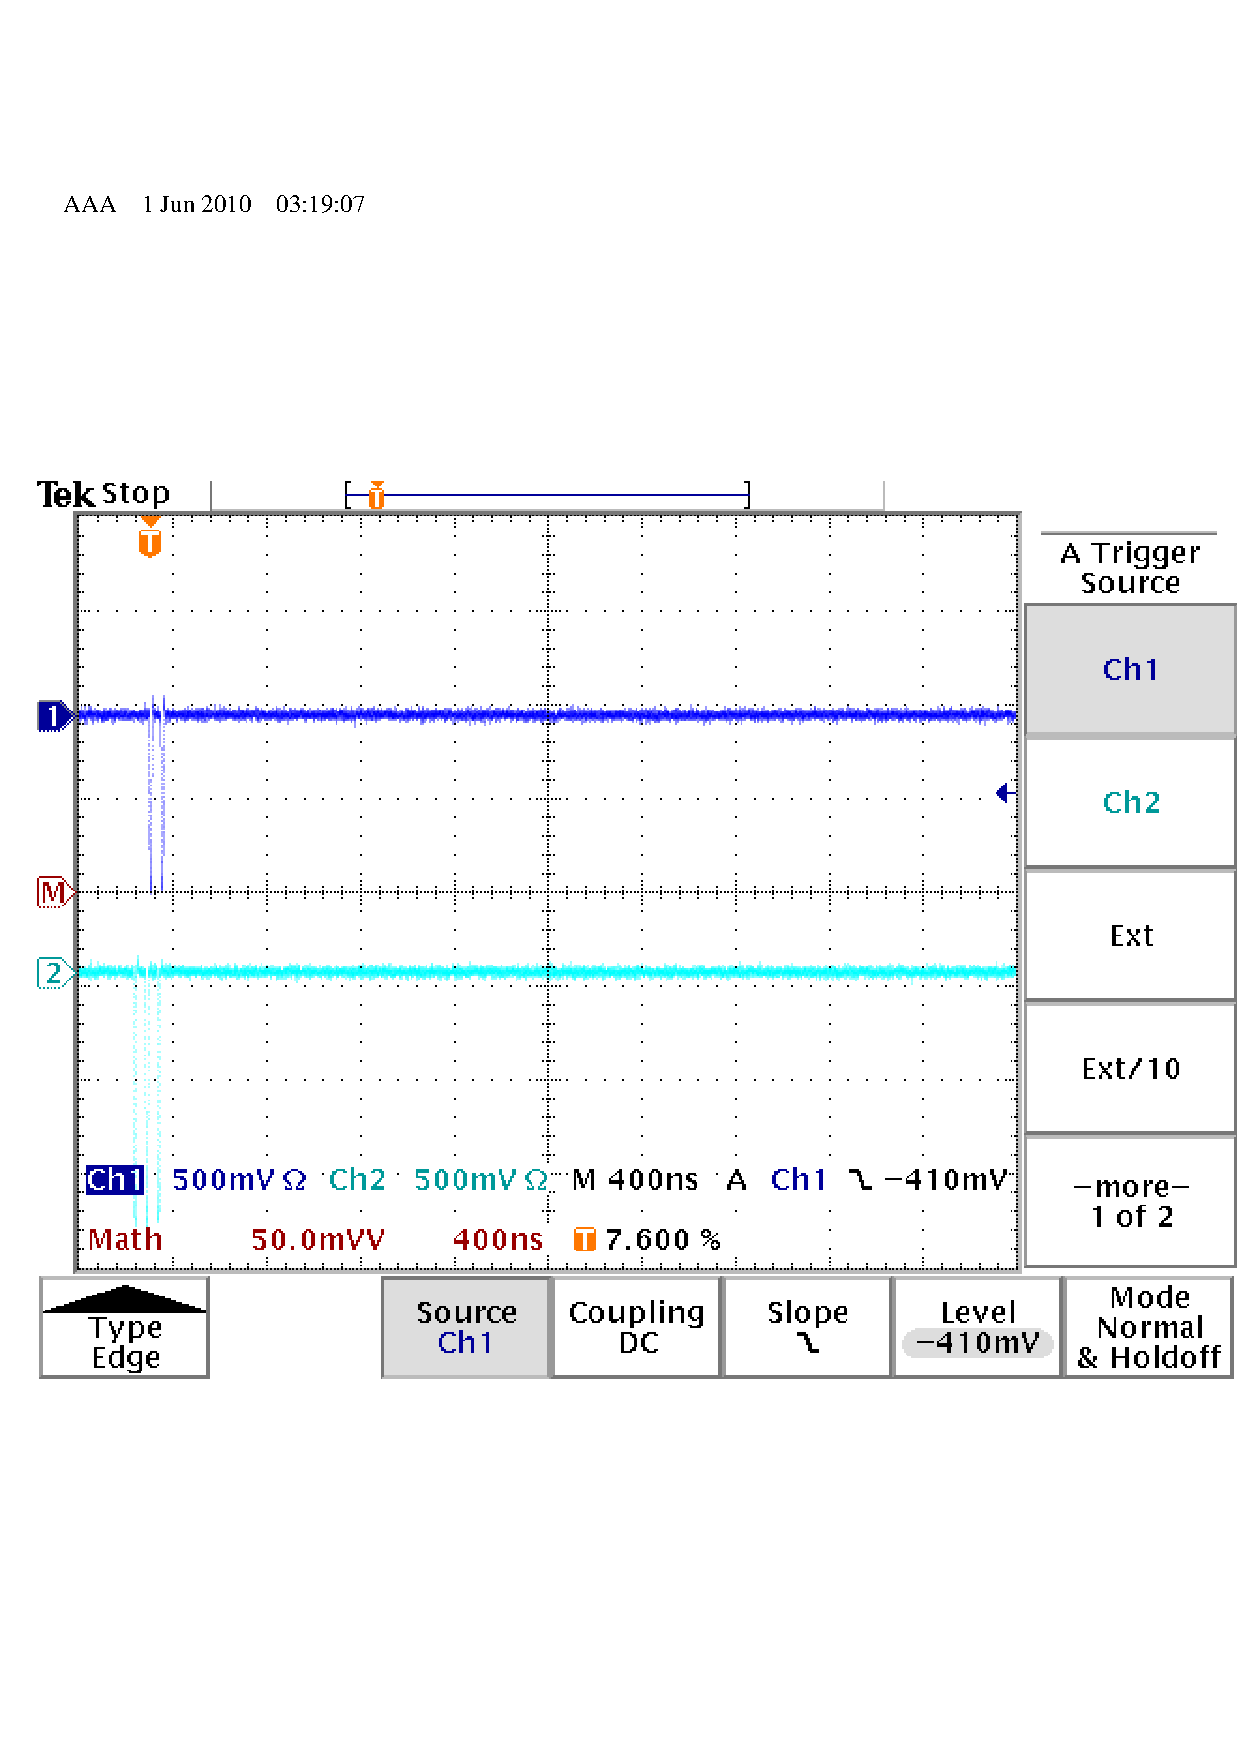
\includegraphics[width=0.45\textwidth,keepaspectratio,viewport=0 52 472 436,clip]{../tmp/TEK000028.pdf}
  }
  \caption{Signale für je einen Szintillationszähler}
  \label{fig:einzelne_SCs}
\end{center}
\end{figure}

\newpage

\section{Quellcode}
\label{sec:sourcecode}

\lstinputlisting[label=lst:source,caption={Makroquelltext}]{../code/muon_tools.C}
% \lstinputlisting[language=Maxima,label=lst:Berechnungen,
% caption={Berechnungen}]{../code/rechnungen.mac}